
%\documentclass[DIV19]{scrartcl}
%\usepackage[paper size={90mm, 120mm},left=2mm,right=2mm,top=2mm,bottom=2mm,nohead]{geometry}
% FIXME try prettyref
\documentclass[oneside,a4paper,12pt,BCOR20mm,DIV14]{scrbook} % should be DIV14
%\documentclass{book}
% this gives a bit more than 2cm margin right and 4cm left
% koma-script.pdf: A4 is 210mmx297mm, BCOR is substraced before the page
% width is divided into DIV parts (HLU), a one sided leaves 1.5 HLU
% HLU*DIV=210-BCOR -> DIV=(210-BCOR)/HLU
% I want BCOR= 20mm 1.5 HLU = 20 mm 
% -> DIV=truncate(190*1.5/20) = truncate(14.25)=14
% I could use headinclude so that the header isn't printed into the margin

% Initially two softbound theses should be submitted to the
% Examinations Office for the examiners. Softbound theses should have
% the pages glued in.
% They don't need gold lettering on the spine.

%\includeonly{spatio-angular}

%\usepackage{enumitem}
%\setitemize{noitemsep,topsep=0pt,parsep=0pt,partopsep=0pt}

%\usepackage{etoolbox}

\pdfminorversion=5
% 9 is best zlib compression i use 0 while writing in the hope that
% git can track changes more easily
\pdfcompresslevel=0
% 3 is maximum for now
\pdfobjcompresslevel=0

\usepackage{booktabs}

\usepackage[utf8]{inputenc}
\usepackage[T1]{fontenc}
\usepackage[usenames,dvipsnames]{color}
\usepackage[onehalfspacing]{setspace} 
%\usepackage[draft]{graphicx}
\usepackage{graphicx}
\usepackage{longtable}
\usepackage{float}
\usepackage{wrapfig}
\usepackage{soul}
\usepackage{amssymb}
\usepackage{amsmath}

%\usepackage{pdfcomment}  % breaks hyperref metadata

% choose font here: http://www.tug.dk/FontCatalogue/mathfonts.html
\usepackage[T1]{fontenc}
%\usepackage[math]{iwona}
\usepackage[math]{kurier}
%\usepackage{cmbright}
\usepackage[scaled]{beramono}

\usepackage{footnote}

\usepackage{microtype}
\newcommand\Small{\fontsize{9}{9.2}\selectfont}
\newcommand*\LSTfont{\Small\ttfamily\SetTracking{encoding=*}{-60}\lsstyle}
\newcommand*\cmafont{\fontsize{8}{8.2}\selectfont\ttfamily\SetTracking{encoding=*}{-60}\lsstyle}


\usepackage{esvect} % vector CB in raytrace chapter



%\newcont\pdfcompresslevel


%\usepackage[hypertex,breaklinks]{hyperref} 
% breaklinks only seems to work with dvipdfm,
% otherwise urls have no
% line breaks

%\usepackage[showrefs,showcites,ignoreunlbld]{refcheck} % for draft, uncomment for final
%\usepackage[notref,notcite]{showkeys}

\usepackage[disable]{todonotes} % for draft, disable for final

\usepackage{lineno}
\usepackage[refpage]{nomencl}
%\special{background Black}\special{color Green}
%\usepackage[utf8x]{inputenc} 
%\usepackage[T2A]{fontenc} % for the russian reference
\usepackage{wasysym} %diameter
% http://www.andy-roberts.net/misc/latex/latextutorial3.html

%\usepackage{url} % natbib.pdf p.11 break urls up, seems to be done
                 % with hyperref, though

\usepackage{natbib}

\usepackage[pdftex,a4paper=true,plainpages,bookmarksnumbered,pagebackref,% put after natbib
pdftitle={Spatio-Angular Microscopy},%
pdfauthor={Martin Kielhorn},%
pdfkeywords={microscopy, photobleaching,%
  phototoxicity, spatial light modulator}, %
pdfsubject={PhD thesis}]{hyperref}


\usepackage{siunitx} %sudo apt-get install texlive-science
\usepackage{units}


% for app_hilo
\usepackage{listings}
\usepackage{color}
\usepackage{textcomp}
\usepackage{subfigure}


% \listfiles % show which files are loaded by tex

\bibpunct{(}{)}{;}{a}{}{,}
\makenomenclature
\newcommand{\vect}[1]{\mathbf{#1}}
\renewcommand{\r}{\vect r}
\renewcommand{\a}{\vect a}
\newcommand{\s}{\vect s}
\newcommand{\vnu}{\mbox{\boldmath{$\nu$}}}
\newcommand{\vmu}{\mbox{\boldmath{$\mu$}}}
\newcommand{\vtau}{\mbox{\boldmath{$\tau$}}}
\newcommand{\vrho}{\mbox{\boldmath{$\rho$}}}
\newcommand{\vvarrho}{\mbox{\boldmath{$\varrho$}}}
\newcommand{\supp}{\mathop{\mathrm{supp}}}
\newcommand{\pois}{\mathop{\mathrm{pois}}}
\newcommand{\step}{\mathop{\mathrm{step}}}
\newcommand{\diag}{\mathop{\mathrm{diag}}}
\def\k{\vect k}
\def\d{\vect d}
\def\e{\vect e}
\def\f{\vect f}
\def\c{\vect c}
\def\x{\vect x}
\def\y{\vect y}
\def\z{\vect z}
\def\q{\vect q}
\def\p{\vect p}
\def\l{\vect l}

\newcommand{\nvect}[1]{\vect{\hat{#1}}}
%\renewcommand{\i}{\nvect i}
\newcommand{\vi}{\nvect \i}
\def\hc{\nvect c}
\def\hs{\nvect s}
\def\hd{\nvect d}
\def\hx{\nvect x}
\def\hy{\nvect y}

\def\hz{\nvect z}
\def\n{\nvect n}
\def\t{\nvect t}
\def\m{\nvect m}
\def\vrho{\boldsymbol\rho}
\def\abs#1{\mathopen| #1 \mathclose|}


\renewcommand{\O}{\textsf{O}} % oxygen

% conclusions of paragraphs in the margin
%\usepackage[marginparwidth=2.5cm]{geometry}
\setlength{\marginparwidth}{2.2\marginparwidth}
\reversemarginpar
\newcommand{\cma}[1]{\marginpar{\cmafont{#1}}}
% include eps or pdf file, that was generated by inkscape, depending
% on if pdflatex or latex processes this file. latex allows a faster
% development cycle but pdflatex generates a smaller and better final
% pdf output
\def\svgending{\ifx\pdfoutput\undefined% 
  .eps_tex% 
  \else%
  .pdf_tex%
  \fi}

% use \svginput{1}{bla} to include bla.svg, make sure you keep this in
% one line, so that make can automatically find the dependencies with
% sed
\newcommand{\svginput}[2]{{\def\svgscale{#1}\input{#2\svgending}}}

\def\pdfending{\ifx\pdfoutput\undefined% 
  _vector.eps% 
  \else%
  _vector%
  \fi}
\newcommand{\pdfinput}[2]{\includegraphics[width=#1]{#2\pdfending}}

% example call \imagw{8cm}{bla.jpg}{bla}{caption abl}
\newcommand{\imagw}[4]{
  \begin{figure}[!hbt]
    \centering
    \includegraphics[width=#1]{#2}
    \caption{#4}
    \label{fig:#3}
  \end{figure}
}

\def\jpgending{\ifx\pdfoutput\undefined% 
  .eps% 
  \else%
  %
  \fi}
% use like this \jpginput{8cm}{imagefile}{caption ...  make sure all
% characters until the opening brace for the caption are on one line
\newcommand{\jpginput}[3]{\imagw{#1}{#2\jpgending}{#2}{#3}}

% this is for plots that are generated by gnuplot
\newcommand{\gnuplotinput}[2]{\begin{figure}[!hbt]%
    \centering%
    \includegraphics{#1_gnuplot}%
    \caption{#2}%
    \label{fig:#1}%
  \end{figure}}

\newcommand{\celegans}{\emph{C.~elegans}}
\DeclareMathOperator{\sign}{sign}
\DeclareMathOperator*{\sinc}{sinc}
\DeclareMathOperator*{\rect}{rect}

% reference to picture
\newcommand{\figref}[1]{\figurename~\ref{#1}}
\title{Spatio-angular microscope} % i don't call make title
\author{Martin Kielhorn}
% short summary at the beginning of a section
\newenvironment{summary}{\begin{quote}\small}{\end{quote}}

\begin{document}
\listoftodos
%\linenumbers
\begin{titlepage}
  
  \hspace{-4cm}
  \svginput{1}{objective-trace}



  \vspace{-5cm}
  
  \hspace{4cm}\textsf{\Huge Spatio--Angular Microscopy}
  
  \vspace{2cm}
  \hspace{6cm}\textsf{\huge PhD Thesis}


  \vspace{3cm}
  \hspace{4cm}\textsf{\Large Martin Kielhorn}
  
  \vspace{1cm}
  \hspace{4cm}\textsf{\Large April 2013}
\end{titlepage}
\newpage
\section*{Abstract}
\begin{summary}
  Photobleaching and phototoxicity pose a problem in live cell
  imaging. Fluorescence imaging induces reactive oxygen species in
  observed organisms which can alter the behaviour of the
  sample. Hence, minimising the light exposure is an important goal.

  We augment a wide field epifluorescence microscope with two spatial
  light modulators. By controlling the spatial excitation pattern and
  the angle of illumination, we can adapt the illumination to the
  specimen. In many cases, this technique will create exposures with
  reduced excitation of the out-of-focus fluorophores, resulting in
  better image quality and less phototoxicity.

  My custom software is used to obtain an initial image stack of the
  specimen. Subsequent image sections are exposed with excitation
  patterns that account for the previous image stack. Depending
  upon the distribution of fluorophores, this adaptive exposure can
  considerably reduce photobleaching and phototoxicity.
\end{summary}

\urlstyle{sf}
%\setcounter{tocdepth}{3}

\chapter*{Preface}
%\section*{Preface}

The work described in this thesis was carried out between June 2008
and April 2013.

In chapter \ref{sec:intro}, we introduce photophysics of fluorescence
and emphasize the importance of oxygen for phototoxicity. Furthermore,
we also explain conventional microscopes and CCD cameras.

In chapter \ref{sec:approaches}, we compare some state-of-the-art
techniques for illumination control in microscopes.  Particularly in
section \ref{sec:light-field-microscopy}, we discuss the micro-lens
based light field microscope by Levoy's computational photography
group, which imaged the toy soldier in 2003.

In chapter \ref{sec:setup}, we describe our microscope and in chapter
\ref{sec:experiments}, we show some images, taken with illumination
control in our prototype.

- ccd measurment

- mapping lcos camera

In the appendix, we also describe a completely different approach for
spatio--angular illumination based on holography (Appendix
\ref{sec:app_holo}) and we document an interferometric attempt to
convert our precise programmable phase mask into a spatial intensity
modulator (Appendix \ref{sec:app_dic}).

Note that the Appendix \ref{sec:dvi} describes a modification of our
prototype with a spatial light modulator that receives data from a
graphics card. A higher bandwidth makes this approach more useful than
the prototype described in the main text and we tried to implement
this first. However eventually, it proved too difficult to trigger the
components in this configuration and we switched to the more
predictable USB-controlled display as described in the main body of
the text.
 
The appendix also contains some theoretical explainations of
raytracing (Appendix \ref{sec:raytrace}), computational optical
sectioning (Appendix \ref{sec:app_hilo}) and the wave-optics based
simulation of our microscope (Appendix \ref{sec:sim-angle}).

\subsection*{Source Code Availability}

Source code that has been developed during this project is available
on \url{https://github.com/plops/mma}.  It contains implementations
for:
\begin{itemize}
\item illumination planning based on raytraces (see Appendix
  \ref{sec:raytrace})
\item moving the $z-$stage of a Zeiss Axiovert 200M microscope body
\item controlling an Andor Clara camera using the Andor SDK version
  2. For the other cameras following below, control software was written:
  \begin{itemize}
  \item Photometrics Cascade~II (interface to unsupported
    closed-source driver, only works on very old 32-bit Linux kernels)
  \item mvBlueFox 102G using the SDK
  \item Logitech Pro 9000 using a generic Video4Linux interface
  \item Andor sCMOS using Andor SDK version 3
  \end{itemize}
\item displaying patterns using a graphics card that supports OpenGL
  on a ForthDD SXGA ferroelectric LCoS display
\item controlling a stand-alone ForthDD WXGA 3DM display controller
  using USB
\item estimating the parameters of a rigid transformation between
  camera and LCoS display (see Appendix \ref{sec:rigid}),
\item controlling the micromirror array by Fraunhofer IPMS using
  their SDK
\item some specific image processing tools:
  \begin{itemize}
  \item three-dimensional convolution and Fourier transforms
  \item drawing of lines and ellipsoids in volumes
  \item rasterization of triangles (for creating shadow maps in the
    BFP, see section \ref{sec:trace-detect})
  \item calculation of optical transfer function for high NA
    objectives
  \item localization of spherical nuclei in volumetric data (parts of
    the algorithm as described in \citet{Santella2010})
  \end{itemize}
\end{itemize}
The main development was done using GNU~Linux. However, portability
was kept in mind and most of the code was made to work with Microsoft
Windows as well.

The drawing on the title page shows the beam path through at
$100\times$ objective with a numerical aperture of 1.45. The design
parameters of the objectives that I used in this project are hard to
come by and I used data from a patent \citep{Matthae2003}.


\subsection*{Acknowledgements}
It is my pleasure to thank all those who have made this thesis
possible. First and foremost, I owe my deepest gratitude to my
supervisor Rainer Heintzmann for giving me the opportunity to become
part of his research group at King's College London and later in the
Institute of Photonic Technology in Jena.

I owe my sincere thanks to Kai Wicker, Jakub Nedbal, Susan Cox, Daniel
Appelt, Ond\v rej Mandula, Ronny F\"orster, Ivana \v Sumanovac,
Eckhard Birkner, Kathrin Klehs and all the other members of our group
for valuable discussions, support and review of the manuscript.

My sincere thanks to the European Union Framework Programme 7 (project
number 2115597) for the studentship on this project.  I also thank
Erhard Ipp, G\"unter Z\"ochling, Vincent Galy, QueeLim Ch'ng, J\"org
Heber, Mark Eckert, Dirk Berndt, Joel Seligson, Jean-Yves Tinevez and
Florian R\"uckerl for helpful collaboration.

Furthermore I highly appreciate the input of Herbert Gross, Miroslav
Grajcar, Edward Rosten, Christophe Rhodes, Paul Khuong, Nikodemus
Siivola, Gabor Melis and Lu\' is Oliveira. Occasionally, the expertise
and insight of them steered me into right direction or greatly
simplified problems I faced.

Finally, I wish to thank the authors and contributors to the following
software projects: Linux, GCC, Emacs, SBCL \citep{Rhodes2008}, Maxima
\citep{Maxima.sourceforge.net2013}, Micromanager
\citep{Edelstein2010}, DIPimage \citep{dipimage}, Wireshark
\citep{wireshark}, Latex, Inkscape \citep{inkscape}, Gimp
\citep{gimp}, ImageJ/Fiji \citep{Abramoff,Schindelin2012} and Blender
\cite{blender}.  These free software projects and their communities
are invaluable to my work and greatly enhance my efficiency.

The work presented in this thesis is my own, unless I cite a
reference.

\begin{flushright}
  M.~K.
\end{flushright}

\noindent
Jena, Germany

\noindent
April 2013
\newpage
\tableofcontents
\printnomenclature
\chapter{Introduction}
\label{sec:intro}
\begin{summary}
  In this work I discuss a modification of a fluorescence microscope    \cma{my device}
  that minimizes the toxic effects of the excitation light.

  In the following introductory chapter I describe what phototoxicity   \cma{phototoxicity}
  is and how it comes about. Then I give an example of how it
  influences biological observations in a developing \celegans\ 
  embryo and describe how this particular biological system can be
  used to evaluate and compare the phototoxicity of different microscopes.

  Later in this chapter I give an overview of image formation   \cma{cameras}
  in the wide-field microscope and I describe its principle limitations
  regarding resolution and depth discrimination. Furthermore I
  discuss the two most important current image detector technologies
  --- electron multiplying charge-coupled devices (EMCCD) and
  scientifc complementary metal–oxide–semiconductor (sCMOS).
\end{summary}
Regardless of whether it is the picture of earth captured by an
orbiting satellite, the x-ray motion picture of a running dog or the
time-lapse recording of a blooming flower. Images capture our
imagination and they are a good starting point to develop new models
and theories.

This is particularly true for microscopy.  Only after people became
aware of microorganisms by direct observation, medieval quack could
finally be overcome and modern medicine based on the scientific
method flourished instead.

Even today --- with electron microscopes, magnetic resonance
tomography and sequencing machines --- optical microscopy still is an
indispensable tool for research of living organisms.

Fluorescence microscopy is of particular importance: It enables the     \cma{labelling, switching}
scientist to selectively label a particular type of molecule in living cells
and observe how they perform their biological function.

Besides localizing molecules it is possible to measure physical
quantities inside of the sample. There are, for example, fluorescent
labels that report membrane potentials or viscosity inside of cells.

Finally, it is even possible to exert a controlling function with the
excitation light: There are compounds that locally release chemicals
when illuminated and there are  genetically encoded ion channels that can be
switched by light \citep{Boyden2005}.

However, the excitation light introduces unnatural and potentially
deleterious energy into the specimen. If the exogenous light harms the
observed organism in any way, this effect is called phototoxicity.

% dennoch: from photophysical prospective of single- and multi-photon
% microcopy, probably the most disheartening reality is the occurrence
% of photobleaching and photodamage
% \citep{diaspro2009nanoscopy}

There are a number of techniques that can reduce phototoxicity: Two
photon excitation, controlled light exposure, selective plane
illumination, highly inclined and laminated optical sheet, and oblique
plane microscopy. I introduce them in
chapter \ref{sec:illum-patterns}. These techniques have different
pros and cons and not all are equally suited for a specific problem,
e.g.\ selective plane illumination is very effective, but it needs two
perpendicular lenses and can not be used for multiwell plates or to
observe the liver of a living, adult mouse.

In this work I present an approach that makes use of modern display
and camera technology. We only modify the microscope's illumination
path, the space around objective lens and specimen remains as
accessible as in any conventional wide-field microscope.



\section{Phototoxicity in life sciences and the model organism
  \celegans}
\label{sec:intro-phototoxicity}
The partner in our project who is responsible for decisions related to
life sciences and biology is Institut Pasteur (Paris, FR). They work
on infectious diseases. 

In order to motivate the importance of phototoxicity, I would like to
portray an elegant drug screening experiment which I have seen on one
of my visits in Paris: An automatic microscope continuously images a
cell culture in multiwell plates. These cells carry a pathogen. The
pathogen, the nuclei of the cultured cells and the membranes of the
cells are each stained with a different fluorophore. The cells in each
well of the plates are exposed to a different chemical.

A chemical is considered a hit and will be investigated during further
trials, when the time lapse images show that the culture cells stay
healthy and the number of pathogens decrease. As neither people nor
animals come to harm, this screening experiment is an impeccable
method to systematically understand and hopefully heal certain
diseases. However, this experiment doesn't work very well, if the
excitation light --- and not the drug --- kills the pathogens. The
effect of phototoxicity should therefore be minimized.


Now one would hardly develop a microscope and directly test it with
dangerous pathogens. As part of our collaboration, the Institut
Pasteur therefore developed a safe biological test system that is
relatively easy to maintain \citep{Stiernagle2006} and allows to test
the phototoxicity of various microscopes \citep{Tinevez2012}.




The basis of the system is the embryo of the organism \celegans. These
are small invertebrates. The adult form is approximately \unit[1]{mm}
long.  Their anatomy and development are comparatively simple and have
been well characterized \citep{Sulston1977,Durbin1987}.

\jpginput{12cm}{celegans-devel}{Phototoxic effects while imaging the
  embryonal development of three \celegans\ embryos (strain
  AZ212, histone-2B tagged with eGFP) with different excitation
  intensities. The embryo with lowest excitation dosage (left)
  develops fastest. The embryo with the highest dosage (right) ceases
  development and nearly all fluorophores are bleached after the
  experiment. Images by J.-Y. Tinevez (Institut Pasteur, Paris, FR).}
  

We use embryos of a genetically modified strain\footnote{Our strain
  has WormBase ID AZ212 \citep{Praitis2001}.} that expresses eGFP
tagged histones (enhanced green fluorescent protein, excitation
maximum \unit[488]{nm}, emission maximum \unit[509]{nm}). Histones are
incorporated into the chromatin during cell divisions, i.e.\ the
nuclei of our worms fluoresce green.  The mother worm passes a
sufficient amount of these proteins into the cytoplasm of the
embryo. In the beginning of its development the embryo entirely relies
on this reserve of histones. Only in a much later stage --- certainly
not during the first few hours, that we observe --- it will form its
own histones.

\figref{fig:celegans-devel} compares time-lapse experiments on three \cma{embryo example} 
different \celegans\ embryos with varying
excitation intensities.

The lineage tree of two developing \celegans\ embryos is the \cma{reproducible development}
same.  With all other factors being equal, particularly if the
temperature is constant at $\unit[21\pm
1]{\degreeCelsius}$, two different embryos will develop at the
same speed from egg to fertile adult in three and a half days.


At the beginning of the experiment, embryos are removed from their
mothers at an identical stage, before any cellular divisions have
occured. Then a $z-$stack of the egg with 41 slices and one micron
$z-$sampling is obtained every two minutes.

The columns in \figref{fig:celegans-devel} depict three different embryos
whose development was imaged according to this protocol for two hours
and 38 minutes with different excitation powers.

The figure displays the maximum intensity projections of the
$z-$stacks.  In order to make the cell nuclei visible in all images, I
normalized the data to the same range. As can be guessed from the
photon shot noise, the upper left image contains the least number of
fluorescence photons, and the upper right the most.

An analysis of the time-lapse data show that one hour into the
experiment the embryo with the highest excitation dose (right) has
stopped developing and its fluorophores are strongly bleached.  Some
cells even turned apoptotic and went into programmed cell death.

After two hours and 38 minutes the experiment was stopped and the
embryo which was exposed to the lowest dose (left) has developed the
largest number of cells. The middle embryo ceased developing while the
right embryo died even earlier and nearly all its fluorophores are
bleached at the end of the experiment.

In \figref{fig:worm-integration-time} I reproduce quantitative data
from \cite{Tinevez2012}. Each data point in this graph corresponds to
a two hour time-lapse imaging experiment of a \celegans\ embryo in a
wide-field microscope. From a very low excitation up to a certain
threshold dose the development isn't affected by the light and
approximately 50 cells develop during the two hours.

For a dose above the threshold the development is slowed due to
phototoxicity and the number of cells at the end of the experiment
decreases.

\gnuplotinput{worm-integration-time}{Longer exposure times are less
  phototoxic. Each data point corresponds to one embryo that developed
  under a particular excitation dose for two hours. The solid lines
  are sigmoidal fits to the data. Also indicated are the two
  phototoxicity thresholds given by the inflection point of the
  sigmoid and their $95\%$ confidence intervals. This data was
  provided by J.-Y. Tinevez (Institut Pasteur, Paris, FR) and is also
  published in \cite{Tinevez2012}.}  

The orange data points in the diagram correspond to a per slice
integration time $\tau$ of \unit[100]{ms} and for the green data
the integration time is five times higher.

\nomenclature{$\Omega$}{Excitation dose in $\joule/(\centi\meter^2\textrm{stack})$} 
\nomenclature{$\Phi_e$}{Radiant flux of excitation light in watts} 
The dose $\Omega$ on the $x-$axis is calculated as
\begin{align}
\Omega = \frac{\Phi_e n \tau}{A},
\end{align}
with integration time $\tau$, area $A$ of the illuminated field, the
number of slices $n=41$ and radiant flux $\Phi_e$ of the excitation
light, as measured in the pupil.

Naively one would assume that it shouldn't make any difference if the
excitation light dose is administered with \unit[100]{ms} or
\unit[500]{ms} exposures but these data show that a longer exposure
time and low intensity are less phototoxic.

These results agree with an earlier study in tobacco plants
\citep{Dixit2003}. They investigate cell death a few days after
illumination and find that there is a threshold dose below which no
phototoxicity can be detected, and that this threshold decreases with
light intensity. Dixit and Cyr show that the damage is caused by
reactive oxygen species and they explain the shift of the
phototoxicity threshold by the limited capacity of the cells'
scavenging system for those radicals. They also predict the existence
of redox-sensitive checkpoints in the mitotic division cycle.

%\citep{Sancar2004}

In summary this section describes how to measure phototoxicity with
biological specimen.  The next section gives an overview of the
underlying photophysics and the rest of this work describes our
attempt to build a microscope with reduced phototoxic footprint.



\section{Photophysical principles of phototoxicity}
\begin{summary}
  Here I give a short overview of fluorescence of molecules in order
  to introduce the terms photobleaching and phototoxicity.
\end{summary}
A fluorophore is a molecule that can absorb and subsequently emit
light. During the absorption of a photon the molecular orbital
transitions from the electronic ground state $S_0$ to an excited state
$S_1$. The lifetime of the excited state $S_1$ is in the order of a
few nanoseconds.
\begin{figure}[!hbt]
  \centering
  \svginput{.8}{flu-level}
  \caption{The Jablonski energy level diagram of an illustrative
    fluorescent molecule. The boxes depict orbitals, up and down
    arrows symbolize the spin of the outer electrons. Fat horizontal
    lines represent electronic states. Thinner lines indicate
    vibro-rotational states. Various processes are shown with their
    typical time scales. VR = vibro-rotational relaxation, ISC =
    intersystem crossing, IC = internal conversion \cite[inspired
    from][]{Haken2006}.}
  \label{fig:flu-level}
\end{figure}
A Jablonski diagram, as depicted in \figref{fig:flu-level}, summarizes
information \cma{energy levels} about the energy levels of a molecule
and possible transition processes.

%  If the photon has an even higher
% energy, the electron will go into the second excited singlet state
% $S_2$.

The majority of known stable and bright fluorophores absorb and emit
in the wavelength range between \unit[300]{nm} and \unit[700]{nm}.
Photons at the high energy end of this range can excite molecules into
higher energy levels $S_n, (n>1)$ than the first excited state; these
states are unstable and hardly return to the ground state $S_0$. On
the other side of the spectrum: a molecule that absorbs in the
near-infrared ($\unit[>700]{nm}$) has a low-lying excited singlet
state $S_1$ and therefore potentially increased reactivity and a high
probability for a non-radiative transfer back into the ground state
$S_0$ \citep{Sauer2011}.


The term \emph{Stokes' shift} describes the frequency shift between
the absorbed and emitted photon; the energy difference is lost as heat
to the fluorophore molecule and surrounding solvent.  For the
practical implementation of fluorescence microscopes this is
significant, as it enables to separate excitation and emission light
with a dichroic beam splitter.

A fluorescence photon is emitted into a random direction. We use this
in the next section to describe image formation in the fluorescence
microscope.


The triplet states $T_n$ play an important role in photobleaching.
Pure electronic absorption of one photon has no effect on the spin of
an electron and therefore the transition from singlet states $S_n$
into the triplet state $T_n$ shouldn't occur. However, interaction
with the nuclei can mediate this spin transition. Therefore, in
fluorophores this transition has a small probability, resulting in
long lifetimes of the triplet state $T_1$.

\cite{Deschenes2002} show that excitation of higher triplet states
$T_n$ is the predominant reactive process for photobleaching in
vacuum. In particular they measured that one rhodamine~6G molecule
\emph{in vacuum} can emit more than \num{1e9} photons before it
bleaches, if the excitation intensity is low enough
$(\sim\unit[1]{\si{\watt/\cm^2}})$ to prevent decay over triplet
states.

In normal atmosphere the prolonged lifetime of the triplet state $T_1$
makes it highly likely for the fluorophore to react with molecular
oxygen $\O_2$. Oxygen is abundant and has a triplet ground state
${}^3\Sigma$ with two unpaired electrons of parallel spin in its
$\pi^*-$orbitals (see \figref{fig:oxygen}).

  \citep{Bernas2004}

\begin{figure}[!hbt]
  \centering
  \svginput{1}{oxygen}
  \caption{{\bf left:} Schematic that depicts how the orbitals of the
    oxygen molecule are formed from the atomic orbitals. {\bf right:}
    Molecular oxygen has the lowest energy in its triplet state
    ${}^3\Sigma$ where the spins of the two outer $\pi^*-$electrons
    are parallel. Inspired from \citet{Linde2011a}.}
  \label{fig:oxygen}
\end{figure}

If a ground-state oxygen molecule comes into physical contact with a
$T_1$ fluorophore, the energy of the latter can be transferred by an
electron exchange energy transfer mechanism in which the orbitals
directly interact with each other \citetext{\citealp[p.~438]{Haken2006} and
  \citealp{Linde2011a}}.

During this reaction, which is also known as triplet--triplet
annihilation, two forms of singlet oxygen form in competition: The
lower energy state ${}^1\Delta$ and the short-lived, higher energy
state ${}^1\Sigma$ that immediately ($T_{1/2}\sim\unit[10^{-9}]{s}$)
sends out a \unit[1268]{nm} photon and decays into ${}^1\Delta$.

The resulting singlet oxygen ${}^1\Delta$ is very reactive. In a
typical specimen it diffuses only a few tens of nanometres until it
reacts with another molecule.

(FIXME 2000 greenbaum measures oxygen production, bernas 2004 anoxia gfp)

Nowadays many methods are known to reduce photobleaching: Substitute
oxygen with noble gases or remove it enzymatically
\citep[p.~89]{Sauer2011}, depopulate the triplet state by adding
reducing as well as oxidizing agents to the solvent
\citep{Vogelsang2008} or couple a triplet quencher directly to the
fluorophore \citep[p.~19]{Sauer2011}. For fixed samples it helps to
change the solvent or polymer.
 
In living specimen these techniques may reduce photobleaching, but
they can also have a detrimental effect on the biological system
itself. Removing oxygen will quite certainly have a negative
effect. In order to reduce phototoxicity it makes sense to think about
the light management in the microscope.


\section{Conventional microscopes}
\begin{summary}
  Most of the fluorescence microscopes that are in common use today do
  not excite fluorophores of the specimen in an optimal way. In
  this section I outline how these microscopes work and explain how
  out-of-focus blur severely limits the performance of the wide-field
  microscope.
\end{summary}


A microscope, is a device that collects light coming from one plane  \cma{lateral image}
and forms a magnified image on a
camera. \figref{fig:widefield-microscope}~b) shows a schematic
representation of the detection path of a wide-field microscope.

The main components are an objective lens with focal length $f$ and a \cma{telecentric arrangement}
tube lens TL1 with focal length $f_\textrm{TL}>f$. Sample, lenses and
camera are arranged in double-telecentric configuration, i.e.\ the
sample is located in the front focal plane of the objective, the tube
lens is at distance $f_\textrm{TL}$ behind the pupil and the camera is
in the focal plane behind the tube lens.


\nomenclature{$\beta$}{Transversal magnification of an objective
  $\beta=f_\mathrm{TL}/f$, for Zeiss lenses the magnification $\beta$
  is written on the objective and the focal length of the tube lens is
  defined as $f_\textrm{TL}=\unit[164.5]{mm}$}


Light from the sample is collimated by the objective lens and
\cma{lateral magnification} re-imaged by the tube lens. The lateral
magnification $\beta$ is given by the ratio of the focal lengths of
the two lenses:
\begin{align}
  \beta=\frac{\overline{O'P'}}{\overline{OP}}=\frac{f_\mathrm{TL}}{f}.
\end{align}
Note that in \figref{fig:widefield-microscope}~b) I represent the
\cma{necessary corrections} objective lens as a single element.  This
is a simplification.

In the paraxial limit ray-tracing calculations for a thick lens or
even several consecutive lens elements can be simplified by bending
the ray only at one place --- at the principal plane.

\nomenclature{marginal ray}{Axial ray through the periphery of the
  entrance aperture}

\nomenclature{chief ray}{Ray from the periphery of the field through
  the center of the entrance aperture}

\nomenclature{entrance aperture}{Projection of the limiting aperture
  of the optical system into object space}


Microscope objectives must collect light from a large aperture in
order to produce a high resolution image. This is a fact I will
support shortly using the wave-optical model. Unfortunately the large
ray angles in the objective prevent its simplified description using
principal planes, but an analysis using the eikonal theory shows that
an optical system that fulfills the Abbe Sine condition allows perfect
imaging even for widespread ray bundles.
\begin{align}
  \beta = \frac{n \sin\alpha}{n' \sin\alpha'} \qquad \textrm{(Abbe Sine condition)}
\end{align}
This condition ensures that the focal length, a quantity which is
usually defined only for paraxial rays, is equal for all angles.  This
in turn means that such a lens carries out a Fourier transform from
the front to the back focal plane with linear scaling. Note that a
lens with a non-linear distortion in the back focal plane will fail to
produce an image that is similar to the object.

It turns out that ray bending in a high-aperture lens system that
fulfills the Abbe Sine condition can be simplified to a one bend at a
single surface, quite similar to the utilization of principal planes
in paraxial optics. For a high-aperture system this surface is no
longer a plane.  Instead it is a sphere with radius $n f$ and called
\emph{aplanatic sphere}. I depict this surface as two circle segments
with bold red strokes on the lenses in
\figref{fig:widefield-microscope}~b).

In addition to the Abbe Sine condition microscope lenses are also
corrected for spherical aberration and linear coma \citep{Gross2005}.
Then the coma rays are symmetric around the chief ray, the wavefront
and point spread function are approximately invariant for small field
sizes (in first order).  This ensures that the imaging conditions are
invariant for small regions of the field plane and allows to express
image formation with linear systems theory.

\subsection{Wave-optical theory for image formation}
In the following I want to describe how the image on the camera       \cma{wave optics}
forms. For this we have to use wave theory because close to the image
rays intersect, invalidating ray-optical predictions. As both
theories are very much related, we can give a useful interpretation of
the aplanatic surface for wave optics.

The underlying Maxwell equations and the wave equation are linear and   \cma{plane waves}
we can represent propagating solutions (evanescent solutions are
neglected) of the wave equation as a superposition of the elementary
solution --- the monochromatic, plane waves described by wave vector
$\k$:
\begin{align}
  u(\r,t)=u\,\exp(i(\k\r-\omega t)),\quad \r=(r_x,r_y,r_z),\
  \k=(k_x,k_y,k_z),\ |\k|=2\pi n/\lambda_0,
\end{align}
The accurate treatment of high-aperture optics would in fact require a
vectorial calculation of the image for a fluorophore with a particular
dipole orientation.  Subsequently these images should be averaged to
account for random fluorophore orientations, but as I don't need
quantitative expressions I limit myself to the simpler scalar problem
which provides a qualitatively similar result.

% \begin{figure}[!hbt]
%   \centering
%   \svginput{1}{sine-condition}
%   \caption{dasfklj}
%   \label{fig:sine-condition}
% \end{figure}



\begin{figure}[!hbt]
  \centering
  \svginput{1}{widefield-microscope}
  \caption{{\bf a)} Transmitted segment of the three-dimensional
    frequency spectrum is highlighted in red on the Ewald sphere. {\bf
      b)} Schematic of the detection path of a modern microscope. The
    sample is in the front focal plane of the objective. The detection
    tube lens TL1 forms a magnified image on the camera. The aplanatic
    spheres for objective and tube lens are indicated in
    \textcolor{red}{red}. {\bf c)} Parallel laser epifluorescence
    excitation. The excitation tube lens TL2 focuses a laser into the
    pupil of the objective. The beam is reflected by a dichroic beam
    splitter (BS) towards the objective. An extended area in the
    specimen is illuminated. Fluorescence light returns through the
    objective, is transmitted through BS and forms an image on the
    camera. }
  \label{fig:widefield-microscope}
\end{figure}

\nomenclature{$u(\r)$}{Scalar field as a function of spatial
  coordinates} 

\nomenclature{$\widetilde u(\vnu)$}{Fourier transform
  of scalar field as a function of spatial frequencies}

\nomenclature{$\r=(r_x,r_y,r_z)^T$}{Three-dimensional spatial
  coordinate} 

\nomenclature{$\r_t=(r_x,r_y)^T$}{Transversal two-dimensional spatial
  coordinate}

\nomenclature{$\vnu=(\nu_x,\nu_y,\nu_z)^T$}{Three-dimensional spatial
  frequency}

\nomenclature{$\vnu_t=(\nu_x,\nu_y)^T$}{Transversal two-dimensional
  spatial frequency}

Assuming excited fluorophores in the sample give rise to a                 \cma{Ewald sphere}
monochromatic electromagnetic field --- again, I simplify the problem
by omitting the complication that fluorophores emit photons in a
wavelength range --- then using the spatial frequency vector
$\vnu=\k/(2\pi)$ we can expand the three-dimensional, stationary field
amplitude distribution $u(\r)$ into its spatial frequency spectrum
$\widetilde u(\vnu)$:
\begin{align}
  u(\r)=\int_{-\infty}^{\infty}\int_{-\infty}^{\infty}\int_{-\infty}^{\infty}
  \widetilde u(\vnu) \exp(2\pi i \r\vnu)\ \textrm{d}^3 \vnu
\end{align}
Since we have assumed a monochromatic field and the length $|\vnu|$ of
the spatial frequency vector is the inverse of the wavelength, the
support of this spectrum $u(\vnu)$ is limited to the surface of a
sphere of radius $n/\lambda_0$:
\begin{align}
  \supp \widetilde u(\vnu) &= \{\vnu \in \mathbb{R}^3: |\vnu|=n/\lambda_0\}.
\end{align}
This sphere is the transfer function of free space, and is also called
Ewald sphere.  \nomenclature{Ewald sphere}{Transfer function of free
  space} Scaling the Ewald sphere with $f\lambda_0$ gives the
aplanatic surface of the lens. 

According to \cite{McCutchen1964} the transfer function $\widetilde
h(\vnu)$ of the lens is defined by complex values on the Ewald sphere. 
aperture:
\begin{align}
  \widetilde h(\vnu)&=P(\vnu_t) \exp\left(\frac{2\pi i}{\lambda} 
    W(\vnu_t)\right)
  \delta\left(|\vnu|-\frac{n}{\lambda_0}\right),
\end{align}
with the Dirac delta function $\delta$, transversal spatial frequency
vector $\vnu_t=(\nu_x,\nu_y)^T$, and the real valued pupil function
$P(\vnu_t)$ and wavefront error $W(\vnu_t)$. McCutchen calls
$\widetilde h(\vnu)$ the generalized aperture.

For this discussion I set $W(\vnu_t)=1$, i.e.\ there are no wavefront
aberration and the lens is diffraction limited. Furthermore I use a
uniform cylinder as pupil function $P(\vnu_t)$, in order to limit the
size of the calotte or cap of the Ewald sphere that is defined by the
acceptance angle $\alpha$ of the objective\footnote{Note that this
  expression is only valid for $\alpha\in[0,\pi/2]$. An expression for
  $\widetilde h(\vnu)$ encompassing the full range $[0,\pi]$ for
  $\alpha$ must contain two functions of each $P$ and $W$, in
  dependence on whether the spatial frequency vector $\vnu$ is
  directed in or against the direction of the optical axis. This is
  necessary to express the transfer function of a 4Pi microscope.}:

% \begin{align}
%   \widetilde h(\vnu) =
%   \begin{cases}
%     P_-(\vnu_t) \exp\left(\frac{2\pi i}{\lambda} 
%     W_-(\vnu_t)\right)
%   \delta\left(|\vnu|-\frac{n}{\lambda_0}\right) & \nu_z<0
%  \\
% P_+(\vnu_t) \exp\left(\frac{2\pi i}{\lambda} 
%     W_+(\vnu_t)\right)
%   \delta\left(|\vnu|-\frac{n}{\lambda_0}\right) & \nu_z\ge 0
%   \end{cases}
% \end{align}

\begin{align}
  P(\vnu_t) &=
  H\left(|\vnu_t|-\frac{n\sin(\alpha)}{\lambda_0}\right), \quad \textrm{with}\ 
  H(x)=
  \begin{cases} 
    1 & x\ge 0 \\
    0 & x<0 
  \end{cases}
\end{align}
where $H(x)$ is the step function. In general $P(\vnu_t)$ can assume
values between 0 and 1 in order to account for apodization due to
Fresnel reflection or natural vignetting. I ignore these effects here.

Multiplication of the angular frequency spectrum $\widetilde u(\vnu)$
with the generalized aperture $\widetilde h(\vnu)$ gives the angular
frequency spectrum of the amplitude in the image:
\begin{align}
  \widetilde u'(\vnu) = \widetilde u(\vnu)\cdot \widetilde h(\vnu).
\end{align}
According to the convolution theorem this multiplication of the
spectra corresponds to a convolution of the field distribution $u(\r)$
and an amplitude point spread function $h(\r)=\mathcal{F}(\widetilde
h(\vnu))$ that describes the imaging of the objective lens:
\begin{align}
  u'(\r) = u(\r) \otimes h(\r) =
  \int_{-\infty}^{\infty}\int_{-\infty}^{\infty}\int_{-\infty}^{\infty}
  u(\r')\ h(\r-\r')\ \textrm{d}^3\r'.
\end{align}


with the
three-dimensional frequency spectrum  of the
sample as shown in \figref{fig:widefield-microscope}~a).




transversal spatial frequencies $\vnu_t=(\nu_x,\nu_y)$

Die Pupille begrenzt die durchgelassenen Strahlbuendel und wirkt damit
als low-pass filter auf das Ortsfrequenzspektrum. Falls das System
Aberrationen aufweist, koennte man diese hier mit der Wellenfront
$W(\vnu_t)$ einfuegn. Durch multiplikation mit der Funktion $\widetilde h$ 

diffraction limited W=1




Faltungstheorem
\begin{align}
  \mathcal{F}[\widetilde h(\vnu_t)\widetilde u(\vnu_t)]
\end{align}


angularly band-limited


\begin{align}
  A &= \frac{f}{d} = \frac{1}{2\tan\alpha}\\
  h_r(\vnu_t,\nu_z)&=\frac{1}{2\pi\nu_t A}\sqrt{1-\left(\frac{2A\nu_z}{\nu_t}\right)^2}
\end{align}

The Ewald sphere allows an intuitive calculation of the transfer
function of a microscope. The low-pass 

The pupil works as a filte




no absorption or diffraction in sample
random fluorophores
recording successive slices, telecentricity, real microscope 
main results: image formation linear in intensity, three dimensionally shift-invariant

missing cone \cite{Streibl1984}


- note that $\nu_z$ can be expressed in terms of the other components,
  replacing in the exponential inside the integral acoordingly gives
  with $= U(\nu_x,\nu_y,\nu_z)/cos(\alpha)$

$$ u(x,y,z)=\int\int U_\textrm{2D}(\nu_x,\nu_y)|_{z=0}  exp(2\pi i (x \nu_x+y\nu_y+z\sqrt{(n/\lambda)^2-\nu_x^2-\nu_y^2})) d \nu_x d \nu_y$$

- the aperture angle $\alpha$ defines the maximum transversal freq of
   the spectrum of a 3d scalar point response function

- the 3d freq spectrum is given by a segment of the ewald sphere
  (which mccutchen calls generalized aperture)

- based on this, one can estimate the transversal distribution of the
  psf I(r,z=0) and the axial psf I(r=0,z)

- first order born approximation:

    - light is deflected only by a single interaction 

    - diffraction is linear in frequency space: diffracted spectrum $U_s$ is
      given by the convolution of the incident spectrum $U_i$ with object
      spectrum f

$$U_s(\nu_x,\nu_y,\nu_z) \sim f(\nu_x,\nu_y,\nu_z) \otimes U_i(\nu_x,\nu_y,\nu_z)$$

    - if $U_i$ is a planar wave, then the scattered wave is just the
      object spectrum shifted by the frequency of the incoming wave

    -single moment transfer: only those frequencies $\vec\gamma$ are
     transferred forr which the laue equation is satisfied

$$\nu_s-\nu_i=\vec\gamma$$





a double telecentric system



the entrance pupil is the the image of the limiting aperture into 

aperture stop limits the direction cosines passing from object space
to image space through the optical system

in a certain distance from the image plane a spherical wave is assumed,
the so-called Gaussian reference sphere


\begin{align}
  \beta = \frac{\nu}{\nu'}=\frac{n\sin\alpha}{n'\sin\alpha'}
\end{align} % FIXME steht da nun n oder nicht? IAT 3

the aplanatic surface and ewald sphere are related just by a factor
$f\lambda$

for application of linear systems theory it is necessary that the
imaging conditions are invariant at least over small regions of the
field plane (isoplanatic condition)

The field in the pupil is
\begin{align}
u(\nu)=F\left[U(x)\right]
\end{align}


The field behind the pupil aperture is
\begin{align}
u'(\nu)=h(\nu) u(\nu)
\end{align}

the field in the image plane is obtained by a repeated Fourier
transform with a corresponding scaling of the pupil coordinates
linear mapping between object and image space coordinates $x'=\beta x$

scaling of the spectra $\nu'=$
\begin{align}
U'(x')=\mathcal{F}(h(\nu) u(\nu)) = H(x) \otimes U(x) = \int U(x'') H(x-x'') \textrm{d}x''
\end{align}

the camera can only detect the intensity
\begin{align}
I'(x')=|U'(x')|^2=U'(x')U'^*(x')
\end{align}

the marginal ray starts from an outer field point in the object and
passes through the center of the entrance pupil, which here is in
this double telecentric system is in axial infinity 

in a system, natural vignetting (projection along chief ray in object
and image) should be taken into account with energy apodization
factors

etendue
geometrical flux



The uncoloured beam in \figref{fig:widefield-microscope}~a) represents
rays that start from the intersection $O$ of the optical axis and the
front focal plane of the objective. The objective collects the rays
and collimates them into a beam that is parallel to the optical
axis. After traversing the tube length $f+f_\mathrm{TL}$, the rays are
focused by the detection tube lens TL1 on the intersection $O'$ of its
focal plane and the optical axis. 

The blue beam corresponds to rays that start from an off-axis point
$P$ in the front focal plane of the objective. Behind the objective
the blue beam is a parallel beam. However, the beam is tilted relative
to the optical axis. The tube lens TL1 focuses the blue beam into a
spot at $P'$ on its focal plane.

The objective fulfils the Abbe sine condition -- it is aplanatic. The
microscope forms stigmatic\footnote{An imaging system collects some of
  the rays, that leave an object and directs them towards the
  image. If all rays that leave an object point converge in the
  conjugate image point, then we call the image point stigmatic.}
images of points from the front focal plane in the plane perpendicular
to the optical axis, containing $O'$ and $P'$. The plane with the
images is called intermediate image plane. It is magnified by the
factor $M$:


In our microscope we use an objective with magnification $M=63$. The
focal length of the tube lens is for most Zeiss
microscopes. Therefore the focal length of our objective is
$f=\unit[2.61]{mm}$.

Let's assume we have an opaque sample with just two small
($\diameter<\unit[120]{nm}$) holes with $\unit[2]{\mu m}$ distance
between them.  We put this object into the front focal plane of the
objective and position a camera on $O'$. When illuminating the mirror
from the side opposite to the objective, the camera will show two
spots with $\unit[126]{\mu m}$ distance.

\nomenclature{NA}{Numerical aperture $\textrm{NA}=n\sin\alpha$, with
  refractive index $n$ of immersion medium and acceptance half-angle
  $\alpha$ of the lens}

Note that \figref{fig:widefield-microscope} depicts a \emph{thin-lens
  model of a high numerical aperture objective} that fulfils Abbe's
sine condition. A real objective contains in the order of ten coated
lenses of different glass and crystalline materials. Their curvatures,
positions and materials were all carefully chosen, taking into account
manufacturing tolerances and wavelengths, so that the microscope
behaves as the thin-lens model predicts. Diffraction at the periphery
of the pupil in the back focal plane dictates the resolution, one can
achieve inside of the sample.


It is quite possible that heating to \unit[37]{${}^\circ$C} will ruin
such a high-precision instrument. A related source of aberrations
(departure of design performance) is the refractive index inside of
the specimen. In Appendix~\ref{sec:ray-aberration} we describe a more
complicated model that can predict the effect of embedding the sample
in water (instead of immersion oil with the same refractive index as
the glass).

\subsection{Widefield epifluorescence microscope}
Fluorescence photons are emitted in all directions, independent of the
original illumination direction. Therefore it is possible and
convenient to use the objective for excitation as well as
detection. This mode of microscopy is called epifluorescence (Greek:
$\varepsilon\pi\iota$; on, above).  In this configuration usually only
a small percentage of the excitation light returns due to diffraction
or reflection. This simplifies the separation of fluorescence light
from excitation light.  Furthermore parts of opaque specimen can be
imaged and it is beneficial that the illumination needs to be aligned
only once.

\nomenclature{BFP}{Back focal plane}

The red beam in \figref{fig:widefield-microscope}~c) is a parallel
laser. The excitation tube lens TL2 focuses the beam into the back
focal plane (BFP) of the objective. The beam is reflected at a
dichroic beam splitter (BS). This is a glass plate that has been
coated with dielectric layers. The refractive index, thickness and
sequence of the layers are designed so that the excitation light is
reflected towards the objective. Excitation light, that is scattered
or reflected in the sample and returns through the objective is
reflected towards the light source. However, lower energy fluorescence
light returning from the objective is transmitted towards the
camera. Behind the objective the beam is parallel and illuminates the
specimen. The field of view is the demagnified diameter of the laser
beam before TL2.
\subsubsection*{Non-uniformity due to coherent interference}
Note that tiny dirt particles and coherent interference in laser beams
can produce unwanted non-uniformities in the illumination. As a remedy
the spatial coherence of the laser is sometimes reduced.  Incoherent
light emitting diodes, mercury or xenon arc lamps are often used
instead of lasers. In the latter case a band pass filter selects the
useful part of the spectrum of the excitation lamp upstream of the
dichroic beam splitter.

\subsubsection{Out-of-focus blur}
However, independent of the choice of the light source, the wide field
microscope in epifluorescence configuration exposes many layers of the
sample. This leads to fluorescence of out-of-focus fluorophores.

There are two reasons, why out-of-focus fluorophores give blurred
images. Not even an ideal imaging system -- a device that forms
%% FIXME refer to maxwell or born/wolf
stigmatic images of all the points in one volume in another volume --
would form sharp images on the camera plane. After all, the camera is
just a plane and the object under observation is three dimensional.

Furthermore a microscope is far from being an ideal imaging system. In
a microscope it is not possible to obtain a sharp image of a different
slice of the object by changing the axial position of the camera
behind the tube lens TL1 \citep{Botcherby2007,Botcherby2008a}.
\subsubsection*{Deconvolution}
When a stack of several slices of an object is obtained, it is
possible to suppress the blurred part of each image in all the
others. These algorithms (deconvolution) can improve the perceived
quality of images in some stacks. However, there are two fundamental
problems:

First the \emph{missing cone problem} prevents focusing on a
homogeneous fluorescent plane. Physics dictates that there is always a
gap in the transfer function of the objective when the fluorescence
process is linear and the objective collects only photons from one
half space (see \figref{fig:missing-cone}). Not all spatial
frequencies within the transfer function attenuate with defocus
\citep{Neil1997}.

\begin{figure}[!hbt]
  \centering
  \svginput{1}{missing-cone}
  \caption{Schematic depicting $k_xk_z-$cross sections of the support
    of optical transfer function (see Appendix~\ref{sec:app_hilo}) for
    microscope objectives with different collection angles. {\bf
      left:} Objectives, that only collect light that is directed into
    one half space, have the missing cone problem. There, low spatial
    frequencies do not attenuate with defocus. {\bf right:} Theoretical
    objective with larger collection angle and no missing cone.}
  \label{fig:missing-cone}
\end{figure}

Second, even with ideal detectors there is photon shot noise in the
image. In deconvolution algorithms the image of one slice is improved
by subtracting blurred versions of the other slices. When the blurred
intensity is large, its shot noise is high as well. Subtraction only
increases noise and a faint in-focus image can be severely
deteriorated by the noise of the out-of-focus light.
\subsection{Confocal microscope}


{\bf c)} Confocal
    microscope. A pinhole PH2 is imaged as a diffraction limited spot
    into the specimen. Returning fluorescence light is only detected
    when it passes through an aligned pinhole PH1. This configuration
    rejects light that doesn't originate from the front focal plane
    (green) of the objective.

One way of addressing both problems of the wide field microscope is
depicted in \figref{fig:widefield-microscope}~c). In the confocal
microscope the whole field of view isn't illuminated simultaneously.
The excitation tube lens TL2 collimates the light coming from a
pinhole PH2 and illuminates the full back focal plane of the
objective. In the front focal plane of the objective the red beam then
converges to illuminate the smallest possible single spot. The spot
size is defined by diffraction at periphery of the BFP. However,
out-of-focus fluorophores are still being excited by the hour-glass
shaped illumination.

The eponymous idea of the confocal microscope is to replace the camera
with a pinhole PH1. This pinhole, if aligned carefully to the position
of the image of the focused laser spot, has no influence on the light
detected from in-focus fluorophores. However, an out-of-focus
fluorophore that is defocused by $\Delta z$ towards the objective will
lead to a diverging beam (colorless) at the tube lens and will be
imaged into a point behind the focal plane of the tube lens. The
pinhole only transmits a part of the circle of confusion. Hence
defocused fluorophores contribute less to the sensor signal.

An image of the in-focus specimen is obtained by scanning the pinholes
PH1 and PH2 over the field of view and measuring intensity at each
position individually. The optical removal of out-of-focus light
prevents degradation of the signal by its shot noise and improves the
point-spread function of the objective. The missing cone problem is
fixed and the resolution improved by a factor of two. Note however,
that information about out-of-focus fluorophores is lost which would
be obtained in a wide field microscope with deconvolution. Therefore a
wide field microscope will give better results when a lot is known
about the sample structure and this knowledge is fed into the
deconvolution. E.g.\ the localization of sparse beads of specific size
will be better in a wide field microscope.

The confocal microscope was invented in 1955 \todo{check patent
  citation} \citep{Minsky1961,Minsky1988} to reduce the influence of
scattering effects in neuron samples stained by Golgi's method. This
invention preceded the laser and was unfortunately not put into
practical use for biology until three decades later \citep{Amos1987}.
\subsection{Phototoxicity in conventional microscopes}
When imaging living specimen we should distinguish between useful and
unnecessary excitation. Taking into account the detection capabilities
of objective lenses we should maximize the ratio of in-focus to
out-of-focus fluorescence. The epifluorescent wide field and confocal
microscope surely do not represent an optimum in this regard.

The following chapter \ref{sec:approaches} will introduce other
microscopy techniques that are more considerate of where to deposit
excitation power within the specimen.
\subsection{2-photon laser scanning fluorescence microscopy}
\label{sec:2-photon}
If the laser intensity in the focal spot of a confocal microscope is
sufficiently high, then two infrared photons can be absorbed within
\unit[$\sim 5$]{fs} and excite the same electronic state.

In this regime, the fluorescence emission increases quadratically with
laser intensity. This non-linearity confines the excitation volume to
the vincinity of the focal plane \citep{Denk1990}. Fluorophores
outside of this region are not excited. Therefore this method produces
sectioned images by default and there is no need for a detection
pinhole.

As an additional benefit infrared light is scattered less than visible
light of half the wavelength. This increases penetration depth and
image quality. Photodamage outside of the focal volume is unlikely and
phototoxicity is much lower, compared to the single-photon confocal
microscope, when $z-$stacks are acquired.

However, the phototoxicity within the focal volume is higher and
techniques like ultramicroskopy (section
\ref{sec:light-sheet-microscopy}) with single-photon excitation are
preferable, when low overall phototoxicity is a requirement.

\section{Image detectors in wide field microscopy}
\label{sec:ccd-intro}
\begin{summary}
  Here we describe CCD\nomenclature{CCD}{Charge-coupled devices}
  sensors and their characteristics.
\end{summary}
Charge-coupled devices are semiconductor devices that contain a 2D
grid of capacitors, formed by at least three groups of electrodes
(phases). Cycling the voltage on these electrodes allows to push
charges, which has been accumulated under the capacitors (registers)
into their neighbours. They turned out to be the ideal tool to move
charges, produced by photon absorption in light sensitive diodes,
across the substrate into read out logic.

Forty years of development lead to imaging devices with remarkable
charge transfer efficiency, high quantum efficiency (up to 95\% with
back illumination) and very low dark currents. Until ten years ago the
performance of CCD imagers in the low light regime was limited by the
noise of the read out amplifier (a few electrons per pixel
rms\footnote{root mean square} \todo{rms}).

Since the millennium we have electron multiplying CCD (EMCCD)
\nomenclature{EMCCD}{Electron multiplying charge-coupled devices}
technology, which allows comparably good performance at low photon
numbers \citep{Mackay,Robbins2003} and moderate read out speeds (tens
of MHz). EM-CCDs contain a row of additional registers in front of the
read out circuit. There, one of the three phases is clocked with a
much higher voltage (up to \unit[40]{V}) then is needed purely for
charge transfer ($\unit[\sim6]{V}$). The large electric fields cause
charge carriers to be accelerated to sufficiently high velocities, so
that additional carriers are generated by impact ionization. The
charge multiplication chance per transfer is small ($\sim1\%$) but by
using several hundred registers a substantial gain in the number of
charges can be achieved. In microscopy we usually work with gains of
up to 300. Higher gains are possible but limit the dynamic range.

The charge amplification helps to push the read noise from
$\sim\unit[40]{electrons\ rms}$ to significantly below
$\unit[1]{electron\ rms}$ --- in effect creating a sensor limited only
by the photon noise. However, the multiplicative nature of the gain
leads to a perceived reduction in the quantum efficiency of the sensor
(excess noise factor), i.e. an image with $\unit[100]{photons/pixel}$
without gain will look like the same image at only
$\unit[50]{photons/pixel}$ with EM-gain (see Appendix
\ref{sec:ccd-meas}).


pixel in
ccd ist passiv
cmos ist aktiv

column parallel readout sony exmor

exmor r additionally back illuminated (only works for small sensors)

%%% Local Variables: 
%%% mode: latex
%%% TeX-master: "kielhorn_memi"
%%% End: 

\comment{
\jpginput{}{led-array}{}
\jpginput{}{myholo}{}
\jpginput{}{phase}{}
\jpginput{}{tf-gpc}{}
\jpginput{}{dunsby}{}
\jpginput{}{aod}{}
}

\chapter{Methods for controlling illumination patterns}
\label{sec:approaches}
\nomenclature{CLEM}{Controlled light exposure microscopy}%
\begin{summary}
  {\color{red} FIXME improve}
  This chapter gives an overview of current microscopy techniques that
  prevent unnecessary fluorescence excitation and thereby reduce
  phototoxicity. In \emph{light sheet microscopy}, an oblique sheet of
  light illuminates the sample without exposing too many out-of-focus
  fluorophores. \emph{Controlled light exposure microscopy} (CLEM)
  takes into account the in-focus fluorophore distribution and
  iteratively improves the signal-to-noise ratio of the measurement.
  Finally, \emph{light field microscopy} allows instantaneous and
  complete control of all parameters of the incoherent light exposure.
\end{summary}
\section{Light sheet fluorescence microscopy}
\label{sec:light-sheet-microscopy}
\begin{summary}
  Light sheets can be directly created with separate optics to
  illuminate the sample from an orthogonal direction. Another
  promising method to create a sheet is to use a high numerical
  aperture objective near the total internal reflection
  angle. Diffraction couples the minimum width of the sheet and the
  extent of the area, where the sheet's width is constant. There is a
  trade-off between sheet width and field of view.
\end{summary}
The idea of illuminating a sample from the side dates back quite far
into the history of microscopy. Already one hundred years ago, an
additional objective, arranged perpendicular to the detection
objective, was used for illumination of the focal plane in the
specimen. This dark field technique was used to characterize gold nano
particles in gold ruby glass \citep{Siedentopf1903}.

Eventually, this illumination method was also applied for fluorescence
microscopy. First, to analyze cochlea specimen \citep{Voie1993} and,
more recently, for the development of embryos
\citep{Huisken2004}. Results in the latter paper have sparked interest
in the technique at many labs \citep{Santi2011}.
\subsection{Light sheet generation with cylindrical lens}
\begin{figure}[!hbt]
  \centering
  \svginput{1}{spim-sketch}
  \caption{Schematic of SPIM (selective plane illumination
    microscope). A cylindrical lens illuminates the specimen with a
    thin sheet of light along the focal plane of the
    objective. Rotating the sample and/or moving it along the axis
    allows to reconstruct a sectioned three-dimensional volume of the
    fluorophore concentration with improved light utilization compared
    to conventional microscopes \citep[inspired from][]{Huisken2004}.}
  \label{fig:spim}
\end{figure}
\figref{fig:spim} shows how the light sheet can be focused into the
specimen using a cylindrical lens. \cite{Huisken2004} employ a water
dipping objective with long working distance (\unit[1\ldots 2]{mm})
and comparatively low NA for detection. A $10\times$ objective with
$\unit[660]{\mu m}$ field of view diameter is used with a sheet
thickness that varies less than $42\%$ ($\unit[6\ldots 8]{\mu
  m}$). The light sheet not only improves sectioning and contrast but
also increases the axial resolution from originally $\unit[14]{\mu m}$
by nearly a factor of two.

\nomenclature{SPIM}{Selective plane illumination microscopy}

The axial resolution of detection objectives with higher numerical
aperture isn't improved so easily over an extended field of
view. Shading effects, diffraction and refraction can deteriorate the
light sheet. As an improvement of the technique it was suggested to
rotate the specimen or illuminate with multiple sheets of light from
different directions.

A major difference between this technique and more conventional
microscopy techniques is the way the sample is mounted. In a normal
microscope, usually, a specimen is placed with a drop of embedding
medium on a \unit[170]{$\mu$m} thick cover slip. Then it is flipped
onto a microscope slide and sealed with nail varnish. This approach of
mounting the sample does not work for an ultramicroscope because there
the sample has to be accessed from two perpendicular sides. Often the
specimen are embedded in an agarose cylinder or sometimes, they are
fixed in a liquid--filled chamber.

\subsection{Light sheet generation using the detection objective}
\label{sec:hilo}
\begin{figure}[!hbt]
  \centering
  \includegraphics[width=12cm]{dunsby}
  \caption{Schematic of oblique plane microscopy (OPM). An index
    matched sample is excited using an oblique plane of light. The
    illuminated plane is tilted relative to the focal
    plane. Therefore, out-of-focus fluorophores on the periphery of
    the field of view are excited as well. Two additional objectives
    in the detection path are used to reconstruct an aberration free
    image of all the excited fluorophores (drawing from
    \cite{Dunsby2008}).}
  \label{fig:dunsby}
\end{figure}
Modern high numerical aperture objectives allow to illuminate an
\emph{index matched} sample with a half angle of up to
$70^\circ$. This enables illumination of an oblique and thin sheet of
light in the specimen just as in selective plane illumination
microscopy. However this technique (oblique plane microscopy, OPM) has
the advantage, that only one objective is used and therefore it will
work with conventional microscope slides. However, one difficulty is
that some of the excited fluorophores are severely defocused in the
intermediate image plane (plane IP1 in \figref{fig:dunsby}). Dunsby
describes how to rotate the observational plane optically in order to
recover an aplanatic image from the oblique illumination plane
\citep{Dunsby2008}. For this, they re-image the sample through two
additional objectives.

\nomenclature{OPM}{Oblique plane microscopy.}

\begin{figure}[!hbt]
  \centering
  \svginput{1}{hilo-sketch}
  \caption{Schematic of rays in HILO (highly inclined and laminated
    optical sheet) technique. The specimen is embedded in a medium of
    lower optical density than the immersion medium. For a very high
    illumination angle --- corresponding to a point on the periphery
    of the back focal plane --- the light would be reflected at the
    ``cover slip-medium'' interface due to total internal reflection
    (TIR). For HILO, a point on the back focal plane slightly closer
    to the optic axis is illuminated. The light enters the embedding
    medium at a highly inclined angle and only a thin sheet in the
    focal plane is illuminated \citep[inspired from][]{Tokunaga2008}.}
  \label{fig:hilo}
  % FIXME the construction of the rays is not correct, they should go
  % to the principal plane and then should be just axially shifted
  % into the aplanatic sphere.
\end{figure}


\nomenclature{TIR}{Total internatl reflection.}

Biological specimen are often not index matched and have a lower index
$n_e\approx 1.33\ldots1.45$ than the immersion oil $n=1.52$. As
indicated in \figref{fig:hilo}, the refraction at the interface
between cover slip glass and embedding medium can be exploited to
illuminate the specimen with a light sheet that is nearly parallel to
the focal plane.  This technique is called highly inclined and
laminated optical sheet microscopy (HILO) \citep{Tokunaga2008,
  Konopka2008}.

\nomenclature{HILO}{Technique for microscopy illumination: highly
  inclined and laminated optical sheet}

Note that the index mismatch between embedding and immersion medium
will introduce aberrations (mostly spherical) in the detection which
will limit the useful imaging depth to a few microns for high aperture
lenses.
\section{Scanning techniques with improved light utilization}
\begin{summary}
  A confocal microscope exposes out-of-focus fluorophores with
  approximately the same dose as the in-focus fluorophores when
  producing and image of a focal slice. During acquisition of z-stacks
  this results in bleaching and successive slice contain less and less
  signal. In particular living organisms may be harmed due to
  phototoxicity during the observation.

  Here I present two methods that can mitigate this effect. The first
  ist the two-photon microscop, in which the excitation is limited to
  the focal plane.

  Furthermore, there is controlled light exposure microscopy that
  selectively illuminates the sample depending on its structure. It
  delivers images with the overall quality as a conventional confocal
  while decreasing phototoxicity and bleaching considerably.

  This method is based on a feedback that controls excitation dose
  depending on the local fluorophore concentration and therefore
  benefits from any latency improvements. In this context I discuss
  two approaches that can increase the scanning speed considerably.
\end{summary}
\subsection{Two-photon laser scanning fluorescence microscopy}
\label{sec:2-photon}
If the laser intensity in the focal spot of a confocal microscope is
sufficiently high, then two infrared photons can be absorbed within
\unit[$\sim 5$]{fs} and excite the same electronic state.

In this regime, the fluorescence emission increases quadratically with
laser intensity \citep{goppert1931elementarakte}. This non-linearity
confines the excitation volume to the vincinity of the focal plane
\citep{Denk1990}. Fluorophores outside of this region are not
excited. Therefore this method produces sectioned images by default
and there is no need for a detection pinhole.

As an additional benefit infrared light is scattered less than visible
light of half the wavelength. This increases penetration depth and
image quality. Photodamage outside of the focal volume is unlikely and
phototoxicity is much lower, compared to the single-photon confocal
microscope, when $z-$stacks are acquired.

However, the phototoxicity within the focal volume is higher and
techniques like ultramicroscopy (section
\ref{sec:light-sheet-microscopy}) with single-photon excitation are
preferable, when low overall phototoxicity is a requirement.
\subsection{Controlled light exposure microscopy (CLEM)}
\label{sec:CLEM}
Im konfokalen Mikroskop wird der Anregungsstrahl in einem rechteckigen
Raster ueber die Fokusebene gescannt. Normalerweise erfolgt dies mit
zwei Galvanometerspiegeln von denen einer die Pixel Spaltenweise
ueberstreicht und der andere (deutlich langsamer) die Zeilen anfaehrt.
Der Anregungslaser ist kontinuierlich aktiv. Letztendlich wird ueber
die Integrationszeit am Detektor das horizontale Sampling definiert.

Das in jedem Pixel gemessene Signal ist proportional zu den
aufgefangenen Photonen und daher mit einem Signalabhaengigen
Quantenschrotrauschen behaftet. Demnach fluktuiert der Signal-To-Noise
Ratio ueber das Bild. Das Bild enthaelt besonders viel Rauschen in
Pixeln mit wenigen Fluorophoren an der entsprechenden Stelle im
Sample. Fuer den menschlichen Beobachter oder viele
Computeralgorithmen ist dieses Rauschen die Bildqualitaet begrenzende
Eigenschaft. Die Tatsache, dass helle Stellen im Sample eine hoeheres
Signal-to-Noise aufweisen, erhoeht die Qualitaet nur
unwesentlich. Prinzipiell waere es vorteilhaft ein Bild mit
Signal-zu-Rausch Verhaeltnis in jedem Pixel zu erzeugen.

Dieser Ansatz wird beim controlled light exposure microscope verfolgt.
Dabei wird jeder einzelne Pixel in eine von drei Klassen
eingeteilt. Je nachdem ob die Zahl der aufgefangenen Photonen zu
Beginn der Integration sehr wenige, sehr viele oder ein Wert
dazwischen sind. Bei den dunkelsten Pixeln (klasse A in fig) geht man
davon aus, dass ueberhaupt keine Fluorophore vorhanden sind und
schaltet den Laser ab. Pixel der Klasse B, die in den ersten Momenten
der Messung nur maessig viele Photonen liefern werden die gesamte
dwell-time ueber beleuchtet. Bei Pixeln der Klasse A mit hoher
Fluorophorkonzentration wird der Laser deaktiviert sobald das
Detektorsignal einen Schwellwert der Photonenzahl ueberschritten
hat. Das Signal ist in diesem Fall nicht die Zahl der gemessenen
Photonen, sondern die Beleuchtungsdauer.

Auf diese Weise erhaelt man ein Bild in dem die hellsten
Fluorophor-Regionen im Bild ein konstantes Signal-Rausch Verhaeltnis
aufweisen. Regionen ohne Fluorophore werden nur sehr wenig
Beleuchtet. Insbesondere bei der Aufnahme von z-stacks macht sich die
Verringerung der Beleuchtungsdosis durch geringeres Bleaching und
verringertee Phototoxicitaet bemerkbar. Die Bildqualitaet nimmt dabei
keinen Abbruch.


The confocal microscope (see \figref{fig:widefield-microscope}~c)
allows another adaptive illumination technique. Each point in the
focal plane of the specimen is treated as one of the following three
cases: point with no fluorophores (A), high concentration of
fluorophores (C) or an intermediate (B).
\begin{figure}[hbtp]
  \centering
  \svginput{1}{clem-sketch}
  \caption{bla}
  \label{fig:clem}
\end{figure}

Ideally, points of type (A) that do not contain fluorophores should
only be exposed until fluorophore content is ruled out. The other two
classes (B) and (C) should be exposed until a fixed number of
fluorescence photons have been detected (C) or a maximum integration
time has been reached (B). Unfortunately, due to the photon nature of
light, sometimes a region of type (B) is incorrectly treated as (A)
which introduces dark pixel artifacts in the image
\citep{Hoebe2010}.

In conventional microscopes, areas of class (C) with high fluorophore
concentration are generally exposed too much. Their signal-to-noise
ratio would be high, but this doesn't increase the perceived image
quality. Furthermore, the regions above and below the focal plane are
unnecessarily subjected to high exposure.

The CLEM approach was first presented by Hoebe et al.\ in
2007,\todo{was that first, get}\ followed by an independent similar
version with adaptive control of the laser power for 2-photon
microscopy by Chu et al.\ \citep{Hoebe2007,Chu2007}.
\subsection{Acousto-optic deflectors for fast beam steering}
In a conventional confocal microscope, the beam is steered by two
galvanometer mirrors. This technique offers very good light throughput
and is sufficient to obtain rectangular images. However, the inertia
of the mirrors severely limit the access rate of spots in the focal
plane.

\begin{figure}[htbp]
  \centering
  \includegraphics[width=12cm]{aod} 
  \caption{Schematic of an acousto-optic deflector (AOD) illumination
    system with $z-$focusing. Figure taken from \citet{Reddy2008}}
% in focusing single s highly preferred http://www.future-perfect.co.uk/grammartips/grammar-tip-focussed-focused.asp
  \label{fig:aod}
\end{figure}


Replacing the mechanical mirrors with an acoustic wave in a
transparent material (TeO$_2$) enables $\unit[4]{\mu s}$ switching
time \citep{Otsu2008} and even allows re-focusing
\citep{Reddy2008}. These acousto-optic deflectors have lower
efficiency than mirrors (70\% for two AODs) and show chromatic
aberrations.

However, as descanning isn't necessary in 2-photon microscopy, the
lower efficiency (in the excitation path) is hardly an
issue. Therefore, this technique for the first time enables ``random
access'' of three-dimensional coordinates in the sample.



\nomenclature{AOD}{Acousto-optic deflector}
\nomenclature{AOM}{Acousto-optic modulator}

% FIXME
\cite{botcherby2012aberration}


\section{Non-scanning techniques}
\subsection{Direct illumination}
An obvious method for doing spatial control is to image a
two-dimensional array of high-power micro-LEDs into the specimen.
\begin{figure}[hbtp]
  \centering
  \includegraphics[width=7cm]{led-array} 
  \caption{An overlay combining wide field micro-LED illumination and
    fluorescence imaging YFP tag expressed in neurons, taken from
    \citet{grossman2010}.}
  \label{fig:led-array}
\end{figure}
However, the problem is to achieve sufficient \emph{irradiance} and
\emph{fill factor}. The angular emission profile of LEDs is often
Lambertian, i.e.\ the back focal plane of the objective would be
over-illuminated and a lot of light would be lost. The fill factor is
limited because it is difficult to put a lot of LEDs close to each
other.  The technique has been demonstrated using a $64\times64$ array
of $\unit[20]{\mu m}$ micro-emitters with $\unit[50]{\mu m}$ pitch
\citep{grossman2010}.  The LEDs can be switched at millisecond speed
and emit at $\unit[(470\pm22)]{nm}$.

\nomenclature{GFP}{Green fluorescent protein}
\nomenclature{EGFP}{Enhanced green fluorescent protein}
\nomenclature{YFP}{Yellow fluorescent protein}
\nomenclature{VCSEL}{Vertical-cavity surface-emitting laser}
\nomenclature{LED}{Light emitting diode} % Fixme
\nomenclature{MMA}{Micromirror array}
\nomenclature{LCoS}{Liquid crystal on silicon (display)}
\nomenclature{DPSS}{Diode-pumped solid-state (laser)}

LED arrays enable interesting experiments where processes are
influenced by light, i.e.\ optogenetics, but the targets ideally have
to be located in the focal plane. Also, it must be verified that the
illumination cone of each LED image doesn't affect the measurement,
i.e.\ activate the specimen in the out-of-focus regions.

Nevertheless, once the LED or VCSEL arrays become available in
interesting spectral ranges, we might see the direct illumination
techniques more often.

\subsection{Intensity modulation}
\subsubsection{Programmable array microscopy}
A technique similar to controlled light exposure microscopy (CLEM,
section \ref{sec:CLEM}) has been implemented in a programmable array
microscope (PAM) \citep{Caarls2011}. Like our microscope, the PAM
images a pattern into the sample using a spatial light
modulator. Contrary to our system, the same SLM is used in the
detection path to recover an image of the in-focus fluorophores.

\begin{figure}[!hbt]
  \centering
  \svginput{1}{pam-sketch}
  \caption{Schematic of a programmable array microscope (PAM)
    \citep[inspired from][]{Verveer1998}. A digital micromirror
    device (DMD) containing an array of tiltable mirrors is imaged
    into the focal plane of the objective. Returning fluorescent light
    from out-of-focus fluorophores is distributed onto both the
    cameras. In-focus fluorescence is only imaged onto camera 1.}
  \label{fig:pam-sketch}
\end{figure}


\nomenclature{PAM}{Programmable array microscopy}%
\nomenclature{DMD}{Digital micro mirror device}%
\nomenclature{MLE-PAM}{Minimized light exposure programmable array microscope}%

\subsubsection{Light field microscopy}
\label{sec:light-field-microscopy}
Interesting work on light fields originally started in the macroscopic
domain of cameras \citep{Lippmann1908%,Sokolov1911
} and was eventually applied as a technique for microscopy
\citep{Levoy2006,Levoy2009,Zhang2009}. This approach is built on
imaging through an array of microlenses.
\begin{figure}[!hbt]
  \centering
  %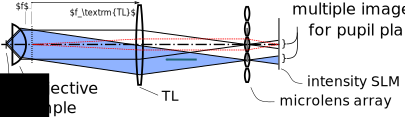
\includegraphics[width=7cm]{microlens-levoy-sketch} %FIXME redraw
  \svginput{1}{microlens-levoy-sketch}
  \caption{Schematic of microlenses in intermediate image plane
    \citep[inspired from][]{Levoy2006}}
  \label{fig:microlens-levoy-sketch}
\end{figure}

A microlens array is placed behind the intermediate image plane (see
\figref{fig:microlens-levoy-sketch}). The light that illuminates one
microlens corresponds to one spot in the focal plane of the
sample. The camera is positioned in the focal plane of the microlenses
and captures an image of the back focal plane behind each microlens
(see red ray bundle in \figref{fig:microlens-levoy-sketch}).

The camera captures the four dimensional light field, leaving the
specimen with spatial coordinates $(s,t)$ and angular coordinates
$(u,v)$. This data enables computational viewpoint shifting,
refocusing, extended depth of field and aberration correction of the
detected fluorescence emission.

\begin{figure}[htbp]
  \centering
  \svginput{1}{microlens-levoy-sketch_2}
  \caption{Construction of an out-of-focus ray bundle through the
    light field microscope. In order to improve the readability of the
    drawing, the magnification in the microscope was set to $1:1$
    (focal lengths of tube lens and objective are equal). An on-axis
    sample point originating from below the focal plane of the
    objective is imaged onto an on-axis point between the tube lens
    and the microlens array. Three of the microlenses re-image this
    on-axis image point into three points behind the plane of the
    camera, i.e.\ the images behind the three microlenses will contain
    bright blurry spots at different positions relative to their
    centre.}
  \label{fig:microlens-levoy-sketch_2}
\end{figure}

\figref{fig:microlens-levoy-sketch_2} shows a bundle of rays
originating from an out-of-focus point. Each of the microlenses that
are hit by the circle of confusion, re-image a fraction of the angular
range into a small image.  This process is crucial because a lot of
the original image information is lost here. The intensities from the
sub-images on the camera can't later be recombined in order to, say,
recover a high resolution image of the defocused point
\citetext{priv.\ comm.\ R.~Heintzmann}.

Additionally the light field microscope doesn't utilize the full
resolution of high-NA objectives. This will prevent the use of this
technique in its current form in the detection path of microscopes.
When the microlenses are small enough, to obtain a high resolution
image of the sample, then the angular resolution diminishes.

However, the same idea can be applied in the excitation path
\citep{Levoy2009}. For illumination purposes, lower resolution will
often suffice. The light-field technique allows unique control of
excitation light intensity and angles at each point of the sample
plane.

\nomenclature{TL}{tube lens}
\subsection{Temporal focusing}
\begin{figure}[!hbt]
  \centering
  \svginput{1}{temporal-focus-sketch}
  \caption{Schematic of temporal focusing \citep[inspired
    from][]{Oron2005}. A grating in the intermediate image plane
    separates the pulse into its spectral components. The out-of-focus
    areas of the specimen are illuminated with a longer pulse. Only in
    the focal plane, all spectral components interfere coherently and
    form a short intensive pulse.}
  \label{fig:oron}
\end{figure}
The axial extent of ultra-short laser pulses can be as thin as a few
microns. A parallel beam can be split into different spectral
components by a grating in the intermediate image plane
\citep{Oron2005}. The tube lens focuses the diffraction pattern into a
line in the back focal plane of the objective.

The objective, which has to be corrected for chromatic aberration and
dispersion, then focuses all the beams onto the focal plane. Different
spectral components arrive in the focal plane at the same time. The
out-of-focus points see an extended illumination. For a high NA
objective, a pulse duration of $\tau=\unit[20]{fs}$ results in slice
of $z\approx\tau c/2\approx\unit[3]{\mu m}$ thickness around the
focus, where the beam has significant intensity.

Using this technique it is possible to build a wide field 2-photon
microscope. That only excites fluorophores within the focal plane. The
technique can be further improved by spatially modulating the beam in
the intermediate image plane for CLEM like performance. This technique
has been implemented in the TF-GPC approach and will be discussed in
the next section.

\subsection{Phase modulation}
\subsubsection{Digital holography}
\begin{figure}[!hbt]
  \centering
  \includegraphics{myholo}\quad
  \svginput{1}{phase-holo_my} 
  \caption{Schematic of spatial illumination by phase holography. A
    phase-only SLM displays a hologram in the plane $P'$ which is
    conjugated to the back focal plane $P$ of the objective
    \citetext{inspired by slide from V. Emiliani}.}
  \label{fig:phase-holo}
\end{figure}
Certain types of liquid crystal spatial light modulators can be used
to modify the phase of light. When such a device is placed into the
back focal plane of a lens, it is possible to control the light
distribution in its front focal plane. An iterative algorithm
(iterative Fourier transform algorithm, IFTA) can be used to establish
a phase image on the liquid crystal display that will result in an
intensity distribution in front of the lens.

\nomenclature{IFTA}{Iterative Fourier transform algorithm}

This approach has been used to excite a two-dimensional pattern in the
specimen \citep{Lutz2008,Zahid2010} and is advantageous especially for
cases where only small parts of the specimen ought to be
illuminated. As opposed to conventional intensity spatial light
modulators, the light can be redirected from dark areas into the
bright areas.

% single photon 405nm uncaging, ifta,
% spherical wave approximation
There is also a limited possibility to create three-dimensional
patterns, e.g.\ several points below, in and above the focal plane by
displaying Fresnel zone planes.  For illumination, usually a laser
with non-zero interference length is employed. However, this
illumination contains an unwanted ``speckle'' pattern in the form of
noisy non-uniformities. To a certain extent, the contrast of the
speckle pattern can be reduced by controlling spatial and temporal
coherence of the illumination (sweeping the frequency of the laser or
changing illumination direction while the detector is integrating).

Holographic control can be used with 2-photon excitation as well
\citep{Nikolenko2008}, % two photon
but this exacerbates the effect of speckles.
\subsubsection{Generalized phase contrast (GPC)}
\begin{figure}[!hbt]
  \centering
  \includegraphics[width=14cm]{phase} % FIXME redraw
  \caption{Schematic of generalized phase contrast
    \citep[from][]{Rodrigo2008}.}
  \label{fig:phase}
\end{figure}
A phase contrast microscope objective \todo{modified ?} can be used to
convert a phase image from the intermediate image plane into an
intensity image in the specimen \citep{Rodrigo2008}\todo{read more of
  this}. Compared to digital holography, hardly any computation is
necessary. Yet, the phase spatial light modulator allows to
concentrate a lot of light even on a small region of the specimen as
opposed to other techniques, which involve intensity modulation and
lose all the light of dark areas by sending it into a beam block or
something similar.

The generalized phase contrast method is suitable even with spatially
incoherent illumination\todo{slightly ?}. However, when the
fill-factor -- the size of the bright area in the image -- changes,
the phase contrast filter must be changed.
\subsubsection{Generalized phase contrast and temporal focusing (TF-GPC)}
The combination of generalized phase contrast and temporal focusing
allows spatially controlled illumination of in-focus areas
\citep{Papagiakoumou2010}. Usage of a phase spatial light modulator
results in high light efficiency compared to intensity modulation.
Splitting and recombination of the spectral components of the pulse
reduce speckle noise considerably.
\begin{figure}[!hbt]
  \centering
  \includegraphics[width=11cm]{tf-gpc} 
  \caption{Schematic of phase contrast with temporal focusing (TF-GPC)
    \citep[from][]{Papagiakoumou2010}, PCF is a phase contrast filter.}
  \label{fig:tf-gpc}
\end{figure}
\nomenclature{PCF}{Phase contrast filter}

%%% Local Variables: 
%%% mode: latex
%%% TeX-master: "kielhorn_memi"
%%% End: 

\chapter{The concept of spatio-angular microscopy}
\label{sec:concept}
\begin{summary}
  Here we introduce our spatio-angular microscope. First we motivate
  the concept of its illumination system using exemplary fluorophore
  distributions, that occur in typical specimen.

  Then we describe some decisions we faced during the initial design
  phase concerning the arrangement of optical components. Furthermore,
  we position our method within known approaches of light control for
  microscopy. Of all published techniques for excitation illumination
  control, the light field microscope \ref{levoy} comes closest to our
  approach.  We explain differences between both techniques and
  discuss their respective pros and cons.  We (FIXME verschieben)
  discuss the peculiarities and limitations of the hardware components
  only in later chapters (\ref{sec:dev1}, \ref{sec:mma}).  Initially,
  the details would be detrimental to clarity.

  It turns out, that the effective use of the spatio-angular
  microscope, requires more knowledge about the specimen than a
  conventional or a SPIM microscope (\ref{spim}). Ideally the
  distribution of refractive index and fluorophores within the
  specimen should be known. If these parameters were known perfectly,
  there wouldn't be any (FIXME) necessity for an image in the first
  place. However, while imaging a known specimen, predictions (FIXME
  gute) of these parameters can often be made. The higher the
  precision of these predictions, the greater the reduction in
  phototoxicity will be.

  The computer-based selection of appropriate illumination masks
  requires the prediction (FIXME), or at least an estimate (FIXME
  understanding), of the three-dimensional distribution of light within
  the specimen.

  In the last part of this chapter, we describe how we practically
  implement the computational control loop in our spatio-angular
  microscope. Here we touch topics of image processing and we also
  draw parallels to treatment planning for radiotherapie of tumors.
\end{summary}
\section{Motivation}

  - Um die grundlegende Idee hinter dem Spatio-Angularen Mikroskop zu
    verstehen, betrachten wir zunaechst die Lichtverteilung im Objekt
    bei einem herkoemmlichen Mikroskop: Abbildung fig:hourglass-all-a
    zeigt schematisch die Seitenansicht von Objektivlinse, Objekt und
    dem Strahlenverlauf des Anregungslichtes in einem konfokalen
    Mikroskop. Ein paralleles Lichtbuendel mit kreisfoermigem
    Querschnitt (in der Darstellung nicht sichtbar) trifft auf die
    Objektivlinse. Die Linse fokussiert das Licht in ihrer Brennebene.

  - Zwischen Linse und Brennebene bilden die Lichtstrahlen einen
    konvergenten Kreiskegel. Angenommen, wir haben eine schwach
    absorbierende Probe, die Energie des Lichtes entlang der
    kreisfoermigen Querschnitte innerhalb des Kegels bleibt dann
    konstant. Die Intensitaet innerhalb des Kegels ist proportional
    zur Dichte der Lichtstrahlen in jedem kreisfoermigen Querschnitt
    und steigt demnach quadratisch an\footnote{Das strahlenoptische
    Modell gilt in grossen Teilen der Darstellung, jedoch nicht
    ueberall.  Das Gesetz von Malus-Lupin besagt, dass die
    Beschreibung mit Lichtstrahlen oder Wellenfronten equivalent sind,
    solange sich Strahlen nicht ueberschneiden (Kaustik) oder (FIXME
    formeln) oder ein starker Intensitaetsgradient auftritt. Demnach
    gilt das strahlenoptische Modell fast ueberall im Kegel, bis auf
    einen Bereich mit einem Abstand von wenigen Wellenlaengen zum Rand
    und im Fokus selbst. Die wellenoptische Behandlung dieser Bereiche
    ist zwar moeglich, rechentechnisch aber erheblich
    aufwaendiger. Deshalb beschraenken wir uns in unserem Prototypen
    und dieser Arbeit ausschliesslich auf das strahlentheoretische
    Modell}.

  - Der fluoreszente Bead (1) im Fokus wuerde demnach deutlich
    staerker angeregt werden, als der Bead (2) ausserhalb der
    Fokusebene. Im konfokalem Fluoreszensmikroskop wird das
    Fluoreszenslicht beider Beads vom Objektiv und
    Detektionstubuslinse in die Zwischenbildebene abgebildet werden.
    Das Bild des in-focus Beads (1) ist dabei scharf, von ihm
    ausgehendes Fluoreszenslicht wird auf einer moeglichst kleinen
    Flaeche konzentriert -- genau auf dem Zentrum des
    Detektionspinholes.  Der out-of-focus Bead (2) erzeugt hingegen
    nur ein unscharfes Bild, sein Licht wird ueber eine grosse Flaeche
    verteilt. Zum detektierten Signal des konfokalen Mikroskops traegt
    zwar nur ein verschwindend geringer Anteil des vom Out-of-fokus
    Beads emittierten Lichts bei, mit Blick auf die Phototoxizitaet
    des Systems kann man jedoch sagen, dass es besser waere, die
    Anregung des out-of-fokus Beads von vornherein zu unterbinden.


\begin{figure}[!hbt]
  \centering
  \svginput{.43}{hourglass-all}
  \caption{{\bf (a)} Two fluorescent beads are illuminated by all
    angles that an objective can deliver. The sharp image of the
    in-focus bead is deteriorated by blurry fluorescence of the
    out-of-focus bead. {\bf (b)} Angular control allows selective
    illumination of the in-focus bead and results in a better image on
    the camera. {\bf (c)} Angular control is insufficient, when an
    extended in-focus area is illuminated. {\bf (d)} However,
    simultaneous spatial and angular control allows sequential
    excitation of the in-focus beads while excluding the out-of-focus
    bead.}
  \label{fig:hourglass-all}
\end{figure}



\begin{figure}[!hbt]
  \centering
  \svginput{1.5}{memi-simple}
  \caption{Simplified schematic of the illumination system in our
    spatio-angular microscope. A homogeneous extended light source
    illuminates from the left. It is imaged by $L_1$ and $L_2$ into
    the intermediate image $F'$. Then the tubelens $L_3$ and the
    objective $L_4$ form an image of $F'$ in the sample plane $F$. The
    first spatial light modulator SLM1 is in the plane P', which is
    conjugate to the pupil (BFP) P of the objective. Using SLM1 we can
    control illumination angles in the sample. SLM2 is directly imaged
    into the sample and allows spatial illumination
    control.} 
  \label{fig:memi-simple}
\end{figure}

\section{A protocol for spatio-angular illumination control}
\section{Finding optimal illuminationOptimization using a raytracer}


\chapter{Device 1: prototype for spatio-angular illumination}
\begin{summary}
   - Im vorhergehende Kapitel haben wir das dem spatio-angularen
     Mikroskop zugrundliegende Konzept dargestellt. Hier gehen wir auf
     zusaetzliche Details ein, die fuer die praktische Implementierung
     wichtig sind. Unter anderem die Eigenschaften der beiden
     verwendeten Displays, elektronische Synchronisation der
     verschiedenen Komponenten und einem Algorithmus, um das             % /Hier mehr spezifische Probleme/
     Koordinatensystem der Kamerapixel und der Pixel des focal plane
     SLM ineinander zu transformieren.

   - Das pupil plane SLM wurde durch unseren Partner Fraunhofer IPMS
     waehrend des Projekts neu entwickelt.  Daher widmen wir uns diesem   % /MMA kommt spaeter extra/
     Subsystem im Kapitel (FIXME) naeher.
\end{summary}
\section{Description of the optical components}
So far we have only shown the beam path for transmissive displays (in
\figref{fig:memi-simple}). Such SLM only have a very low transmission
in practice. Therefore we use reflective displays in our prototype.

In \figref{fig:memi-real} I adjusted the beam path accordingly. This
schematic also depicts the optics we use to adapt light from the laser
to fill the etendue of our system. The light source enters the system
from the bottom left. The optic components are color corrected and
have anti-reflex coating for wavelengths in the range from
\unit[400]{nm} to \unit[700]{nm}.

The system successively illuminates the pupil plane SLM---a grayscale
micromirror array developed by our project partner Fraunhofer IPMS
Dresden---and the focal plane SLM, a commercial binary liquid crystal
on silicon display.
 
I gathered some of the following details from the documents that were
created during the development of our prototype and are classified as
confidential. I have summarized the key decisions here and the
relevant project partners have agreed to the publication (FIXME not
finished).


\begin{figure}[!htbp]
  \centering
  \svginput{2}{memi-real}
  \caption{Schematic of the light path through our microscope. Laser
    light enters from the lower left, is scrambled and homogenized to
    illuminate the pupil plane SLM in P'' and the focal plane SLM in
    F'. $F$ is the field plane in the sample and its primed versions
    are conjugated planes. $P$ is the pupil of the objective. $B_0$
    and $B_1$ are adjustable circular apertures. PBS is a polarizing
    beam splitter. DBS is a dichromatic beam splitter.  The red boxes
    deliminate subsystems of the illumination system: {\bf A:} light
    scrambling and homogenization, {\bf B:} Fourier-optical filter to
    provide intensity modulating pupil plane SLM. {\bf C:}
    Polarization based intensity modulator as focal plane SLM. {\bf
      D:} Wide-field fluorescence microscope with detection
    path. (FIXME finish diagram, don't use B twice)}
  \label{fig:memi-real}
\end{figure}

\subsection{Ensuring homogeneous illumination}
A quantitative evaluation of our experiments (FIXME ref sec:results)
with different illumination patterns is simplified when both pupil
plane SLM and focal plane SLM are uniformly illuminated.

We use either a laser\footnote{Lasever LSR473H, diode-pumped solid
  state laser, output power 600mW, $\lambda=\unit[473]{nm}$} or an
light emitting diode (LED) \nomenclature{LED}{light emitting diode} as
the light source in our experiments. Below we discuss optical measures
that attain homogeneity of the illumination of both displays.

The LED\footnote{Huey Jann HPB8-48KBD, wavelength
  $\unit[(463\pm1)]{nm}$, brightness \unit[35]{lm}, view angle
  $120{}^\circ$, FIXME TODO: Flaeche messen} we use has a large active
area. Due to etendue mismatch a relatively large amount of its
produced light will never reach the sample. But it is easy to achieve
a homogeneous illumination. Moreover, the LED can be quickly switched
on and off electronically \footnote{The DPSS Laser doesn't allow fast
  direct electronic switching at full power. We have to use an
  acousto-optic modulator connected with the additional expense of its
  optical alignment (FIXME siehe spaetere ref section).}.

Unlike an LED, a laser delivers light of considerably higher spectral
radiance ($\unit[]{W/(sr\, m^2 m)}$). Thus it is in principle possible
to use the laser as a highly efficient light source for our
system. Unfortunately, the high spectral and spatial coherence of a
laser often lead to high-contrast fluctuations of the irradiance and
we have to compensate for this by time averaging.

When using the Laser, we send its parallel Gaussian beam into a
bundle\footnote{Fiber bundle with circular cross-section (Loptek,
  Berlin, DE), \unit[1.1]{mm} diameter and \unit[2]{m} length. The
  beam broadening is $3{}^\circ$ and increases, when the bundle is
  bent \citep{D8.4}.}  of randomly distributed fibers. This randomizes
the light distribution at the bundle output and also broadens the
illumination angles.

A relay system (A1) images the circular output of the fiber bundle
onto the entrance of a light pipe. This relay system contains a
rotating microlens array\footnote{Array of cross-oriented cylindrical
  lenses on both sides with a pitch of \unit[0.5]{mm} resulting in an
  effective focal length of \unit[6.9]{mm} (LIMO, Dortmund, DE).}. It
is driven by a motor with the axis of rotation being diplaced from the
optical axis. This time-varying element allows to reduce speckle.

Both, the fiber bundle and microlens array, increase the etendue of
the laser illumination to the optimum value, which is given by one of
our SLM as discussed below in \ref{sec:etendue} (FIXME ref). 

The light  pipe is  a hollow  mirror-integrator tunnel  with quadratic
cross-section and depicted in \figref{fig:integrator-rod}. The mixing
effect of the  tunnel can be understood by  considering the irradiance
in the plane of the tunnel output as it would occur without tunnel.

Drawing the outline of the square cross-section into this irradiance
map selects the light that directly reaches this plane.  Surrounding
this outline with the four squares that touch its edges selects the
light that will reach the output plane after one reflection. The
irradiance maps from neighbouring squares are mirrored and added to
the direct illumination. Depending on the numerical aperture of the
input light, more reflections may occur --- resulting in the addition
of irradiance from next-nearest-neighbours and so forth.

This improves the uniformity of the light distribution in the output
plane without altering the numerical aperture of the light.  The more
subregions are superimposed, the better will be the uniformity.
Assuming $N$ subregions were overlaid and their contributions were
statistically independent, then according to the central limit theorem
the standard deviation of the irradiance is proportional to
$1/\sqrt{N}$ \citep{Koshel2012}.

However, we also align the source distribution to be rotationally
symmetric about the optical axis and obtain an even more uniform
output than this prediction because positive and negative slopes from
different subregions compensate in the superposition (also
\cite{Koshel2012}).

In our system the side length 

ueberaus
prohibitively 

Eine Relais-Optik (A1
   und A2 in Fig 4.1) vergroessert
   den Tunnelausgang des Tunnels auf $\unit[4\times4]{mm^2}$
   in die Ebene F'''.

\footnote{Ein Tunnel mit $\unit[4\times4]{mm^2}$
   Querschnitt beduerfte nicht dieser Optik, dann waeren die Winkel
   der Strahlen im System jedoch noch kleiner und der Tunnel muesste
   unhandlich lange werden.} 

   \jpginput{8cm}{integrator-rod}{Hollow mirror-integrator tunnel with
     a quadratic cross section of \unit[2.5]{mm}
     side length and \unit[250]{mm} length.}



 - Zu den zwei Relais-Systemen hat der Optikdesigner kommentiert
   (FIXME ref D8.9), dass diese nicht fuer eine perfekte Abbildung,
   sondern fuer einen guten Transport der homogenenen Lichtverteilung    % /Interessantes zu Relais-Systemen an Tunnelenden/
   optimiert wurden. Beim System A1 am Tunneleingang werden drei Elemente
   (FIXME oder 2?, und wo ist das Mikrolinsenarray) eingesetzt, um das
   Licht vom runden Faserende in den quadratischen Tunneleingang zu
   transportieren. Am anderen Ende (A2 Fig 4.1) transportieren fuenf Elemente das
   Licht vom Tunnelausgang in die Ebene F''' mit der
   Beleuchtungsapertur.

 - Waehrend der Konzeption wurde auch eine auf zwei Mikrolinsenarrays    % /Nicht benutzt alternative/
   (fly's eye condensor) basierende Optik fuer die Homogenisierung des Lasers in
   Betracht gezogen (FIXME ref D8.2). In-Visions Planung zufolge,
   waere dieser jedoch schwieriger zu justieren als der Tunnel und
   zudem nicht fuer den vollen Wellenlaengenbereich von 400 bis 700nm
   verwendbar gewesen.

  - Um eine homogene Ausleuchtung mit dem Tunnel zu erreichen sind       % /Erfahrungen/
    folgende Punkte wichtig (FIXME ref D8.5):

   - Das Buendelende sollte den Tunneleingang deutlich ueberdecken. Es
     muss vermieden werden, dass die Tunnelecken dunkler als die Mitte
     des Tunnels sind. Ein inhomogen ausgeleuchteter Buendeleingang
     fuehrt zu inhomogener Beleuchtung des pupil plane SLM.

   - Das Ende des Faserbuendels muss in vier Achsen justiert werden
     koennen (Zentrierung von Position und Winkel).

   - Die Brennweite der Mikrolinsen sollte kuerzer gewaehlt werden,
     als die Rechnung vorhersagt. Damit kann unweigerlich auftretendes
     Mikrochipping der zementierten Glasspiegel kompensiert werden.

\subsection{ Fourier-optischer Filter zur Kontrasterzeugung am pupil plane SLM}
  - Der micro-mirror array, den wir als pupil plane SLM einsetzen,        % /MMA torsion spiegel/
    besteht aus Torsionsspiegeln, die die Phase des Lichts modulieren
    (fuer eine genauere Beschreibung siehe spaeteres Kapitel               
    FIXME). Um damit eine Intensitaetsmodulation zu bewirken, nutzen
    wir den in Fig 4.2 B gezeigten Fourier filter. 

  - Die Linse L1 hat zwei Aufgaben: Zum einen bildet sie die Feldmaske   % /Schlierenoptiklinse/
    B0 in den Feldstopp B1 ab. Zum anderen wird die Ebene P'' mit dem
    SLM nach unendlich abgebildet.

  - Bei ungekippten Spiegeln, wird somit F''' nach F'' abgebildet und    % /MMA Kontrasterzeugung/
    gleichzeitig gibt es ein scharfes Bild von P'' nach P'. Beide
    Ebenen F'' und P' sind dann homogen ausgeleuchtet.

  - Werden die Spiegel auf der linken Haelfte in P'' gekippt, dann
    lenken sie das Licht entlang der gestrichelten Linie (in Fig 4.1)
    ab. Dieses Licht wird von der Apertur B1 absorbiert und steht dann
    nicht in P' zur verfuegung. D.h. die rechte Seite in P' ist
    dunkel. Der gesamte radiant flux ($\unit[]{W}$) durch die Apertur in
    F'' nimmt ab, die irradiance ($\unit[]{W/m^2}$) ueber die Apertur
    bleibt aber homogen.

  - Im realen System besteht die Linse L1 aus 4 Elementen. Aufgrund
    der Symmetrie weist sie keinen axialen Farbfehler auf. Es bleibt
    jedoch ein kleiner lateraler Farbfehler (FIXME genauer ergruenden
    was das bedeutet).
 

\subsection{ Relais-System zwischen pupil plane und focal plane SLM}
  - Die Linsen L2 und L3 bilden ein doppelt telezentrisches             % /Relais-System/
    Relais-System mit Vergroesserung 2 und bilden F'' auf der Ebene
    des focal plane SLM in F' ab. Gleichzeitig bildet dieses
    Relais-System den pupil plane SLM von P'' nach unendlich ab.
 
  - Prinzipiell koennte man auch den focal plane SLM in F'' an Stelle
    der Apertur B1 platzieren. In unserem Prototypen haben wir uns
    jedoch fuer dieses zusaetzliche Relais-System entschieden, um den
    Kontrast beider SLM voneinander zu entkoppeln.

   - TODO warum haben wir das relay system? 
     - vermutlich weil wir den mma kontrast vom lcos entkoppeln wollen
     - es ist natuerlich fuer sammelnde system, dass axial color sich
       aufaddiert und nicht kompensiert wird


\subsection{ Polarisationsbasierte Kontrasterzeugung am focal plane SLM}
  - Der von uns verwendete focal plane SLM ist ein liquid crystal on
    silicon Geraet, dass die Polarisation des reflektierten Lichts
    entweder um 90 grad dreht oder konstant laesst.
 
  - Ein Polarisationsstrahlteiler erzeugt daraus einen binaeren
    Intensitaetskontrast (siehe Fig 4.1 C).

  - Wir haben uns fuer einen wire-grid Polarizer (Moxtek PBF02C, Orem,
    UT, US) entschieden, weil die Platte weniger Rueckreflexe
    verursacht als ein Strahlteilerwuerfel.

  - Die s-Polarisation des eingehenden Lichts wird in Richtung des SLM
    reflektiert. Aktive Pixel des SLM rotieren die Polarisation des
    Lichts um 90 Grad und passiert dann den Strahlteiler als
    p-Polarisation in Tranmission in richtung Mikroskop. Dort befindet
    sich ein zusaetzlicher Cleanup-Analysator im Strahlengang.
 
  - Es waere auch denkbar, SLM und Strahlteiler anders anzuordnen, so
    dass das vom SLM kommende Licht in das Mikroskop
    \emph{reflektiert} wird. In diesem Fall verschlechtert jedoch eine
    ungewollte Oberflaechendurchbiegung des Strahlteilers die
    Abbildungsqualitaet vom focal plane SLM. Deshalb nutzen wir den
    Strahlteiler in Tranmission.

  - Die duenne Platte (<2mm) des Strahlteilers macht das System leicht
    asymmetrisch und fuehrt damit hauptsaechlich zu Astigmatismus und
    lateral color (ref D8.9 FIXME), das Optikdesign bleibt aber
    beugungsbegrenzt.


\jpginput{14cm}{setup-photo-blueprint}{The wide field epi-fluorescence
  microscope with attached illumination head. The positions of the two
  spatial light modulators (Micro mirror array (MMA) and liquid
  crystal on silicon display (LCoS)) are indicated. Drawing by Josef
  Wenisch (In-Vision, Austria).}


\jpginput{14cm}{memi-setup-only-lenses}{only lenses7}

\subsection{ Variables Teleskop als Tubuslinse}
  - Die groesse der Pupille von Mikroskopobjektiven haengt von deren
    Bildfeld und numerischer Apertur ab. Die letzt Linse
    TL${}_\textrm{ill}$ in unserem Beleuchtungssystem ist daher so
    konzipiert, dass sie P'' mit variabler Vergroesserung nach P
    abbildet. 

  - Die Linse besteht aus drei beweglichen Gruppen und kann somit
    garantieren, dass der pupil plane SLM bei Vergroesserungsaenderung
    stationaer auf der pupil plane des Objektivs abgebildet bleibt und
    gleichfalls der focal plane SLM immer im unendlichen abgebildet
    bleibt (FIXME gibt es ein paper mit begruendung?).





\begin{figure}[!htbp]
   \centering
   \svginput{2}{memi-sketch}
   \caption{Schematic of the lenses in the MEMI system and their focal
     lengths. The focal length $f_\textrm{TL}$ of the tube lens can be
     varied. This allows to scale the second intermediate image
     $r''_\textrm{MMA}$ of the micro mirror array to fit the back
     focal plane of different objectives. Dimensions in mm.}
   \label{fig:memi-sketch}
 \end{figure}




% \imagw{14cm}{mma}{{\bf left:} Scanning electron microscope image of
%   the micro-mirror array (MMA).  The pixel pitch of the device is
%   \unit[0.016]{mm}. The hinges for the tilt movement and the
%   electrodes are clearly visible. {\bf middle:} Optical reflective
%   microscope image of the MMA. {\bf right:} exaggerated rendering of
%   how a 8x8 checker board pattern would be displayed on the
%   device. Electron and optical micrograph by Fraunhofer IPMS Dresden
%   (Germany)}

% \begin{figure}[!hbt]
%   \centering
%   \includegraphics[width=7cm]{mma-plain}
%   \includegraphics[width=7cm]{mma-ill}
%   \caption{{\bf left:} Micro mirror array chip during installation of
%     the optics. {\bf right:}~Illuminated micro mirror array in the
%     aligned system.}
%   \label{fig:mma-closeup}
% \end{figure}

%\chapter{optimization of the spatio-angular illumination patterns}
%\label{sec:optimization}
%\chapter{mma as an intensity modulator}
%\label{sec:mma}
%\include{mma}
%\include{device2}
% ~/from-hp2-notebook/0331/lens
% there is also code
\chapter{Raytracing for spatio-angular microscopy}
\label{sec:raytrace}
\renewcommand{\i}{\nvect i}
\begin{summary}
  Imaging with the microscope we developed requires a continuous
  update of the patterns for the spatial light modulators during
  operation. It is not easily possible to solve the problem with
  commercial software. Therefore, a simple raytracer is implemented in
  this work.

  This chapter documents the basic concepts. Some approximations,
  which are usually used in optical design (paraxial, only non-skew
  rays) are not applicable here, because rays are to be pursued in all
  possible angles through diverse fluorophore distributions in the
  specimen.

  I begin by introducing simple geometric formulas to determine the
  points of intersection between a ray and a plane or a sphere. I also
  describe how to calculate refraction at a planar surface.

  Then I explain the refraction at a thin, paraxial lens and show a
  modification of the formulas for high aperture lenses. This allows
  to trace rays through a microscope objective in two directions
  (denoted as detection or illumination direction) without knowing the
  exact design parameters and glass types.

  Furthermore, I consider the refraction at the ``cover slip--medium''
  interface for non-index matched media. This enables the calculation
  of illumination patterns for highly inclined and laminated optical
  sheet microscopy, as introduced in section \ref{sec:hilo}.

  I follow up with a rather technical discussion of a geometric
  problem that helps to significantly speed up the raytracing
  calculations for the specific case of a sample that can be
  represented as a three-dimensional distribution of fluorescent
  spheres.

  {\bf Note:} The formulas that are emphasized by surrounding frames
  are implemented in the computer code that is published on
  \url{https://github.com/plops/mma/tree/master/lens}.
\end{summary}
\section{Basic geometric algorithms}
\subsection{Intersection of a ray and a plane}
 \begin{figure}[!hbt]
   \centering
   \svginput{1}{plane-intersection}
   \caption{Schematic of plane-ray intersection.}
\end{figure}
Let a ray start at a point $\s$ with direction $\hd$.  A plane
(defined by a point $\c$ and the unit normal $\n$) intersects this ray if
its normal and the ray's direction are not perpendicular:
$\n\,\hd\not=0$. The distance between the plane and the origin is
$h=\c\,\n$. The equation of the plane is given in Hesse normal form:
\begin{align}
  \r\n=h
\end{align}
I replace the coordinate $\r$ with the ray equation and solve for the
parameter $\tau$.
\begin{align}
  (\s+\tau\,\hd)\,\n&=h\\
  \s\n+\tau\,\hd\,\n&=h\\
  \tau&=\boxed{\frac{h-\s\,\n}{\hd\,\n}}
\end{align}
The point of intersection is located on the ray at $\s+\tau\,\hd$.
\subsection{Intersection of a ray and a sphere}
Let a ray start at a point $\s$ with direction $\hd$.  Let a sphere be
centred in $\c$ with radius $R$. There are two equations
\begin{align}
  (\r-\c)^2&=R^2\\
  \r&=\s+\tau\hd
\end{align}
that define the intersection points. By substituting $\r$ one obtains
a quadratic equation in the distance $\tau$ along the ray:
\begin{align}
  (\s+\tau\hd-\c)^2&=R^2\\
  \l&:=\boxed{\s-\c}\\
  l^2+2\tau\l\hd+\tau^2-R^2&=0\\
  \underbrace{1}_a\tau^2+\underbrace{2\l\hd}_b\tau+\underbrace{l^2-R^2}_c&=0
\end{align}
%\subsubsection{Solving the quadratic equation to obtain the ray--sphere intersection}
In order to prevent numerical errors the following solution should be
used \citep{Press1997}:
\begin{align}
  \Delta&:=\boxed{b^2-4ac}\\
  q&:=\boxed{-\frac{b+\sqrt{\Delta}\sign b}{2}}\\
  \tau&=\boxed{
  \begin{cases}
    q/a &\,\textrm{when}\,\abs{q}\approx 0\\ 
    c/q &\,\textrm{when}\,\abs{a}\approx 0\\
    (q/a, c/q) &\,\textrm{else}
  \end{cases}}
\end{align}
If the discriminant $\Delta$ is negative the ray misses the sphere and
there is no solution. If the discriminant is zero the ray touches the
periphery of the sphere and there is only one solution. A positive discriminant
corresponds to two solutions.
\subsection{Refraction at planar surface}
Now I describe the refraction at a planar surface\footnote{I use the
  same notation as \cite{McClain1993}.}. The wavelength of the light
in vacuum defines the length of the wave vector $\k_0$. The lengths of
the incident and transmitted wave vectors $\k_1$ and $\k_2$ are
obtained by multiplication with the refractive index in their
respective half space:
\begin{align}
  k_0&=2\pi/\lambda\\
  k_1&=n_1 k_0\\
  k_2&=n_2 k_0.
\end{align}
\begin{figure}
  \centering
  \svginput{1}{refraction}
  \caption{Refraction at an interface transforms the incident wave
    vector $\k_1$ into the outgoing wave vector $\k_2$.}
  \label{fig:refraction-plane}
\end{figure}
I choose the normal $\n$ to be directed into the half-space of the
incident wave (see \figref{fig:refraction-plane}) and define the
transversal and normal component of the wave vectors to be:
\begin{align}
  \k_{1n}&=(\k_1\n)\n\\ 
  \k_{1t}&=\k_1 - \k_{1n}.
\end{align}
These two vectors are orthogonal and during refraction the transversal
component of the wave vector is invariant:
\begin{align}
  k_2^2&=k_{2n}^2 + k_{2t}^2\\
  \k_{2t}&=\k_{1t}.
\end{align}
Using the two equations from above, one can calculate the length of
the normal component of the transmitted wave vector $\k_2$:
\begin{align}
  k_2^2&=k_{2n}^2 + (\k_1 - \k_{1n})^2\\
  k_{2n}^2&=k_2^2-(\k_1-(\k_1\,\n)\,\n)^2\\
  &= k_2^2-(k_1^2-2(\k_1\,\n)^2+(\k_1\,\n)^2)\\
  &= k_2^2-k_1^2+(\k_1\,\n)^2.
\end{align}
Finally, one can express the full transmitted wave vector $\k_2$ using
only known quantities:
\begin{align}
  \k_2&=\k_{1t}-\sqrt{k_2^2-k_1^2+(\k_1\,\n)^2}\n\\
  &=\k_1-(\k_1\n)\n-\sqrt{k_2^2-k_1^2+(\k_1\,\n)^2}\n. \label{eq:k2}
\end{align}
I divide by $k_2$ with $\k_2/k_2=\t$ and $\k_1/k_2=\eta\,\i$ in order
to introduce unit direction vectors $\i$ and $\t$ for incident and
outgoing light. The relative index change across the interface is
$\eta=n_1/n_2$. With these substitutions equation (\ref{eq:k2}) becomes:
\begin{align}
  \t&=\eta\,\i-\eta\,(\i\,\n)\,\n-\sqrt{1-\eta^2+\eta^2\,(\i\,\n)^2}\,\n\\
  &=\boxed{\eta\,\i-\left(\eta\,\i\,\n+\sqrt{1-\eta^2(1-(\i\,\n)^2)}\right)\n}
\end{align}
When the expression under the square root is negative a reflection
occurs instead  of refraction. Note that in my application total internal
reflection (TIRF) just corresponds to a loss of the beam, because the reflected beam no longer
contributes to sample illumination. The exact direction of this
 beam is not relevant in this case but I give the equation here for
completeness' sake.

In the case of reflection, the tangential component is invariant and
the normal component inverts sign:
 \begin{align}
   \k_2&=\k_{1t}-\k_{1n}\\
   &=\k_1 - 2\k_{1n}\\
   &=\k_1-2(\k_1\,\n)\,\n\\
   \t_\textrm{TIR}&=\boxed{\i-2(\i\,\n)\n}
 \end{align}
\section{Refraction through lenses}
An \cma{validity of thin lens model} ideal lens is infinitesimally
thin and is completely defined by its focal length. For an ideal lens the focal
length is independent of the incidence angle but in practice, the
model of the thin lens is only valid for lenses of long focal length and
for paraxial rays that subtend very small angles from the optical
axis.

For a better approximation of refraction through a \cma{principal planes} thick lens
the two principal planes of
the thick lens are calculated and the ray is shifted between them axially
\citep{Smith2000}. The principal plane of a thick lens is located on
the intersection between an incident beam $\i$, that is parallel to
the optical axis, and the transmitted beam $\r$. Just as the focal
length, the principal planes are a property of lenses that are only
defined in the paraxial limit. There are always two principal planes,
one for each of the two possible illumination directions. The
distances between each principal plane and its corresponding focus
point (the intersection of $\r$ with the optical axis) are identical,
and define the focal length.

As already mentioned in section \ref{aplanatic} on page
\pageref{aplanatic} a microscope objective is a lens which is
corrected to have a constant focal length for rays of widely varying
incidence angle. In this case, the principle surface is no longer a
plane but is deformed into a spherical surface. After introducing the
formulas for the thin lens in the next section, I show in section
\ref{sec:high-aperture-lens} how to carry over those formulas to a
model that describes an aplanatic lens with immersion.

\subsection{Refraction through a paraxial thin lens}
First I describe the refraction by a thin lens: The incident beam with
direction $\i$ hits the lens at the point $\vrho$. A line parallel to
$\i$ through the centre $O$ of the lens defines the point on the focal
plane, which will be intersected by the transmitted ray $\r$ as well.


\begin{figure}[hbtp]
  \centering
  \svginput{1}{lens-fwd}
  \caption{Construction of a ray that is refracted through a thin
    lens. The incident beam with direction $\i$ (from right) hits the
    lens at the point $\vrho$. This diagram is inspired from a figure
    in \cite{Hwang2008}.}
\end{figure}


The red triangle~1 with the points $ABC$ is similar to green
triangle~2 with points $FOA$. All three angles are identical because
each of the lines are parallel: $\overline{CB} \parallel
\overline{OA} \parallel \vrho$, $\overline{FA} \parallel
\overline{CA}$ and $\overline{AB} \parallel \overline{OF} \parallel
\i$. The side $\overline{OF}$ is hypotenuse of the yellow right angled
triangle 3. Its adjacent with respect to the angle $\theta$ has length
$f$. Therefore one can deduce the length
$\abs{\overline{OF}}=f/\cos\theta$.



Between the two similar triangles, the following relation 
can be used to calculate the length $\abs{\overline{BC}}$:
\begin{align}
  \frac{\abs{\overline{BC}}}{\abs{\overline{BA}}}&=
  \frac{\abs{\overline{OA}}}{\abs{\overline{OF}}}\\
  \frac{\abs{\overline{CB}}}{1}&=
  \frac{\rho}{f/\cos(\theta)}.
\end{align}
Given its length, the vector $\vv{CB}$ is now calculated by its length
and the direction $\vrho$. With this vector and $\i$ one can now
obtain the (arbitrarily scaled) transmitted vector $\r'$.  Only the
two framed equations need to be implemented to calculate refraction on
a thin lens with the procedure from above:
\begin{align}
  \vrho&=(x_0,y_0,0)^T=\rho (\cos\phi,\sin\phi,0)^T\\
  \phi&=\arctan(y_0/x_0)\\
  \cos\theta&=\boxed{\i\,\hz}\\
  \r'&=\i- \frac{\cos\theta}{f}\vrho\\
  \r&=\boxed{\frac{f}{\cos\theta} \i -\vrho}
\end{align}
with the axial unit vector $\hz=(0,0,1)^T$.
\subsection{Refraction through high aperture objective (illumination)}
\label{sec:high-aperture-lens}
Now I modify the results of the calculation from the previous section
to treat an aplanatic immersion objective \citep{Hwang2008}.
\begin{figure}[!hbt]
  \centering
  \svginput{1}{obj-fwd}
  \caption{Ray construction for a high numerical aperture objective
    with immersion. As opposed to a thin air lens the objective's
    focal length needs to be corrected by the focus difference vector
    $\a$ to accommodate for the immersion and one must take into
    account spherical principal surface (aplanatic surface).}
\end{figure}
I account for the immersion medium by axially shifting the focal plane
in sample space to $nf$ using the difference vector $\a$, i.e.\ in an
immersion medium with $n=1.52$ the focus moves further away from the
principal plane.
\begin{align}
  \a &= \boxed{f (n-1) \hz} \\
  R &= \boxed{nf}
\end{align}
In order to account for the curvature of the aplanatic surface, the
origin of the transmitted ray is axially shifted by a $\rho-$dependent
sag $\s$ from the principal plane onto the aplanatic surface:
\begin{align}
  \s &= \left(R - \sqrt{R^2-\rho^2}\right) \hz
\end{align}
The final ray exiting the objective has the direction $\r_0$:
\begin{align}
  \r_0 &= \boxed{\r + \a - \s}.
\end{align}

All microscope lenses that come into consideration for use in the
system that we built are designed as an aplanatic lens. The model
described by above formulas is therefore very well suited to represent
the objectives when we run our illumination optimization algorithm to
find illumination patterns for the two SLM in our spatio-angular
microscope.

In the paper \citet{Hwang2008} the authors demonstrate the viability
of this model by comparing its results with a full raytrace through a
$100\times$ objective with $NA=1.4$. There, focus displacement errors
are less than \unit[130]{nm} for a field of $\unit[86.4]{\mu m}$
radius. This is perfectly adequate for our application.

One might think it would be better to know the exact objective
parameters, i.e.\ glasses, curvatures and vertex positions of lens
surfaces. These details are, however, to my knowledge not published by
any manufacturer. In addition alignment of the components plays a
prominent role in building high performance objectives. Therefore just
the design parameters alone probably do not provide a better model of
a microscope objective. They would have to be augmented with
performance measurements of the individual objective,
e.g. point-spread functions in different regions of the field.

\subsection{Reverse path through oil objective (detection)}
Now I consider an oil immersion objective in the detection direction,
tracing rays from the sample into the pupil.

For that I present two approaches. The first and simpler one utilizes
the fact that a perfect microscope lens converts ray angle in the
sample in a linear manner into positions on the pupil. This approach
is sufficient when calculating pupil plane SLM patterns for samples in
an index matched embedding medium.

In the second approach I additionally calculate the angle in which
rays emerge from the pupil. For a perfectly aplanatic lens this would
hardly be an advantage but the formulas will be modified to take into
account aberrations.
\subsubsection{Easy case: back focal plane positions only}
If the points of ray intersection of the back focal plane are
sufficient, a full raytrace is not necessary. This is the case with
aberration-free imaging, i.e.\ when the sample is embedded in an index
matched medium and we want to calculate a pattern for the pupil plane
SLM. Then it is possible to ignore the starting points of rays in the
specimen and just work with their directions.

A unit ray direction $\i=(x,y,z)^T$ in sample space is transformed
into a position $\r_b=(x',y')^T$ in the back focal plane of the
objective. The azimuthal angle $\phi$ isn't changed when going through
the objective. The polar angle $\theta$ defines how far off axis the
back focal plane is hit.
\begin{align}
  \phi'&=\phi=\arctan(y/x)\\
  \theta&=\arcsin(\sqrt{x'^2+y'^2})\\
  \r_b&=r_b\,(\cos\phi',\sin\phi')^T,\quad\textrm{with}\   r_b=nf\sin\theta
\end{align}
 \begin{figure}[!hbt]
   \centering
   \svginput{1}{obj-rev}
   \caption{Schematic for tracing a ray direction $\i$ from sample
     space into the back focal plane. The bigger the angle between
     $\i$ and the optical axis, the further outside the ray will pass
     through the back focal plane.}
 \end{figure}
 \subsubsection{Full raytrace through oil objective in detection
   direction}
\label{sec:objective-raytrace-detection}
Now I discuss the general case and calculate both the origin and the
direction of a ray emerging from the back focal plane. This is
necessary in order to trace light bundles from the specimen into the
plane of the camera (or focal plane SLM). In the next section I will
further modify these formulas to incorporate aberrations due to
non-index matched embedding medium.

The position of the objective is defined by its principal point $\c$
and the normal $\n$ (directed along optical axis towards sample
space). The incident ray is defined by its starting point $\p$ and the
direction $\i$. First I calculate the centre of the aplanatic sphere
$\vect g$ (see \figref{fig:obj-rev-full}).
\begin{align}
  \vect g &= \c + nf\, \n.
\end{align}
\begin{figure}[!htbp]
  \centering
  \svginput{1}{obj-rev-full}
  \caption{Construction to find the transmitted ray through an oil
    immersion objective from a point within the sample.}
  \label{fig:obj-rev-full}
\end{figure}
Then I obtain the position $\p'$ by intersecting the incident ray and
the plane perpendicular to the optical axis through the centre
$\vect{g}$ of the aplanatic sphere.  The focus difference vector $\a$ is
defined by its length and the optical axis. It can be used to
calculate an intermediate point $\p''$.
\begin{align}
  \a &= -f\, (n-1)\,\n \\
  \p'' &= \p' + a.
\end{align}
The point $\p''$ has been shifted, so that an aplanatic air lens would
image it exactly as the oil objective would image $\p'$. One can use
$\p''$ to find the direction $\t$ of the transmitted ray. It is just
the normalized difference vector $\vect m$ to the principal point $\c$.
\begin{align}
  \vect m &= \c - \p'' \\
  \t &= \vect m / \abs{\vect m}.
\end{align}
As a last step I calculate the starting point $\e'$ of the transmitted
ray by intersecting the incident ray with the aplanatic sphere (in
point $\e$) and axially shifting this point onto the principal plane.

Note: In order to verify the correctness of these formulas or their
implementation it is possible to compare the algorithms of this
section (for tracing in detection direction) and section
\ref{sec:high-aperture-lens} (for illumination direction).
\subsection{Treatment of aberration (detection)}
\label{sec:ray-aberration}
Now I will extend the formulas of the previous section to include
aberrations due to a non-matched embedding medium $n_e\not=n$.

I consider a ray originating in point $\p$ with direction $\i$ within
an embedding medium of index $n_e$. I determine the intersection $\f$
of the ray with the ``cover slip--embedding'' interface and refract to
obtain $\i'$. Then I calculate the time $t$ a photon takes, to travel
from $\p$ to the interface $\f$:
\begin{align}
  t = \abs{\f - \p} \frac{n_e}{c}
\end{align}
and extend the path of the photon backward along the direction $\i'$
(corrected for the refraction at the ``cover slip--embedding'' surface) by
the distance $tc/n$. This results in the corrected position $\p'$ that
indicates where the photon would have originated if the embedding
medium were index matched.  Now I can apply the equations from the
previous section on the ray defined by $\p'$ and $\i'$ to obtain the
transmitted ray in the pupil.

 \begin{figure}[!hbt]
   \centering
   \svginput{1}{obj-rev-full-emb}
   \caption{Construction of an oil immersion objective with a
     non-index matched embedding medium.}
 \end{figure}
\section{Sphere projection}
\label{sec:sphere-projection}
While the previous sections have described a fairly general raytracer,
this section is very technical and relates to the specific problem to
represent a fluorophore distribution as a model of spheres and
simulate it with as few rays as possible.


\begin{figure}[htbp]
  \centering
  \svginput{.95}{touch-cone}
  \caption{{\bf (A,B,E)} Diagrams depicting the geometry of a sample
    of spherical nuclei. The main text derives the rays on the cone
    through the target point $\c$ that touches an out-of-focus nucleus
    in the curve $C$. {\bf (C)} Map of the pupil plane. A ray is sent
    from each point of the pupil plane into the target point $\c$. The
    brightness value in the pupil map indicates the length of the
    segment of the ray that intersects out-of-focus nuclei. {\bf (D)}
    Approximation of the map in (B) using the technique discussed in
    this section with a minimum number of rays per out-of-focus
    nucleus. }
  \label{fig:touch-cone}
\end{figure}


\figref{fig:touch-cone}~A) shows two rays emanating from the pupil
plane and illuminating the target point $\c$. For
\figref{fig:touch-cone}~C) rays were traced from each point of the
pupil plane through the target point $\c$. The brightness of the map
in \figref{fig:touch-cone}~C) indicates the length of ray segments for
rays that intersect with out-of-focus rays.

Creating such an image in the illumination direction requires to trace
a lot of rays (at least $50\times 50$). In order to reduce the
computational effort, I reverse the calculation direction and trace
rays starting from the periphery of out-of-focus nuclei through the
target point $\c$ in order to determine appropriate ``shadow masks''
in the pupil plane (as depicted in
\figref{fig:touch-cone}~D)). Already with six rays per nucleus, this
approach can determine very good masks.

Now I explain how to select good points on the periphery of
out-of-focus nuclei in order to allow this calculation. I utilize the
geometry in \figref{fig:touch-cone}~E).


The tangents of an out-of-focus sphere
{\color[rgb]{0.06666667,0.50196078,0}$S^\s_r$} centred at $\s$ with
radius $r$ that pass through the target $\c$ form a double cone
(assuming $\c$ is outside of $S^\s_r$). The tangents touch the surface
of the sphere $S^\s_r$ in the circle
{\color[rgb]{0.66666667,0,0}{$C$}}. We will find a parametric
expression for the points on the circle $C$ by intersecting the sphere
$S^\s_r$ and the sphere {\color[rgb]{0.28235294,0.24313725,0.21568627}$S^\c_R$}
centred at $\c$ with radius $R=\abs{\c-\s}$ which is the distance from
the target to the centre of the out-of-focus sphere.

In order to find a point $\e$ where a tangent touches the out-of-focus
sphere, it is sufficient to solve the following equation in a
two-dimensional coordinate system with the origin in the centre $\s$
of the out-of-focus sphere:
\begin{align}
  (x-R)^2+y^2&=R^2\\
  x^2+y^2=r^2
\end{align}
There are two solutions:
\begin{align}
  x_1&=\frac{r^2}{2R}\label{eqn:x1}\\ 
  y_{1/2}&=\pm\frac{r}{2R}\sqrt{4R^2-r^2} \label{eqn:y1}
\end{align}
In the case $R\le r$ the out-of-focus nucleus is very close to the
target, obviating the reason to do the projection in the first
place. In the more useful case of $R>r$ there are two solutions but
either one of them is sufficient to define the circle $C$.

I construct two normalized vectors $\hx$ and $\hy$ that span the
coordinate system, in order to transform the solution from 2D into
3D. The direction of $\hx$ is given by the difference vector between
target $\c$ and nucleus centre $\s$. The direction $\hy$ must be
perpendicular to $\x$ and I ensure this by calculating the cross
product of $\x$ with an arbitrary vector $\vzeta$.  The only
constraint on the vector $\vzeta$ is that it must not be colinear with
$\x$. Therefore I choose $\vzeta$ to be a vector along the $z-$axis,
except when $x$ comes close to the $z-$axis. Then I choose $\vzeta$ to
be along the $y-$axis.
\begin{align}
  \x&=\c-\s\\
  \y&=\x\times\vzeta \quad \textrm{with}\ \vzeta=\begin{cases}
    (0,0,1)^T & \textrm{when}\ \abs{x_z}<\frac{2}{3}\abs{\x}\\
    (0,1,0)^T & \textrm{else}
  \end{cases}\\
  \hx&=\x/\abs{\x}, \quad \hy=\y/\abs{\y}
\end{align}
Now I can sample the intersection circle $C$ in order to create
viable starting points $\e$ for tangential rays.  Let $M_\phi^\hc$ be
a rotation matrix that rotates a vector by angle $\phi$ around an axis
$\hc$. A point $\e$ on the circle is then defined using one solution
from equations (\ref{eqn:x1}) and (\ref{eqn:y1}). The ray direction $\f$
is then easily obtained:
\begin{align}
  \e(\phi)&=\s+x_1\hx+y_1M_\phi^\hx\,\hy\\
  \f(\phi)&=\c-\e.
\end{align}
Tracing a sufficient number of rays (e.g.\ 7) with direction $\f$ for
different angles $\phi$ to the back focal plane gives the projection
of the intersection circle $C$. Note that this projection in general
is not a circle anymore.

For practical reasons I project the vector $\hx$ as well. I use it as
a centre to rasterize the shape in the pupil plane as a fan of
triangles.

\section{Conclusion}
In this chapter I have given an overview on the raytracer that I use
as a component in the illumination optimization algorithm for the
spatio-angular microscope. This software is tailored to the problem of
imaging with an aplanatic lens. I optimized the calculations so that
illumination patterns can be determined in real time, while the device
operates.

I described an algorithm that can account for aberration that occurs
when a sample is not embedded in index matched medium. On the one hand
this has a negative impact on the resolution of the detected images
already for small penetration depths ($\sim\unit[10]{\mu}$) but it
enables the interesting approach of highly inclined and laminated
optical sheet microscopy (see section \ref{sec:hilo}). In this case, a
window on the edge of the pupil is illuminated so that rays approach
the ``cover slip--medium'' surface close to the critical angle of total
reflection --- and after refraction they will traverse the medium in a
very steep angle. To illuminate the proper position in the field, the
window that is displayed on the focal plane SLM must be moved in order
to compensate for any, but mainly spherical, aberrations.

Note that ray optics are not a sufficient approximation, when
intensity features in the scale of the wavelength are to be
investigated. Small features would mean that only a few pixels of the
focal plane SLM would be enabled. This would mean that information of
the pupil plane SLM pattern is heavily filtered and no simultaneous
tight angular control would be possible. Therefore, algorithms that
are based on code in this chapter must generate patterns with big
feature sizes. Features on the pupil plane SLM should be larger than
several percent of the pupil diameter.

%FIXME maybe compare to ./cyberpower-store/0314/zeiss-patents/20080106795-correction-ring.pdf 
%or US7268953-63x.pdf


%%% Local Variables: 
%%% mode: latex
%%% TeX-master: "kielhorn_memi"
%%% eval: (reftex-mode)
%%% eval: (flyspell-mode)
%%% End: 


\chapter{Experimental results with spatio-angular microscope}
\label{sec:results}
\begin{summary}
  Ich beschreibe eine Experimente die die Funktion unseres
  Prototypen unter Beweis stellen.

  Im ersten nutze ich die total internal reflection aus, die Auftritt,
  wenn das Sample in einem Medium mit geringerer Brechzahl als der
  Immersion eingebettet ist. Damit kann ich auf einfachen weg zeigen,
  dass die Winkelbeleuchtung funktoiniert.

  In einem weiteren Experiment messen wir das Beleuchtungsfeld im
  Sample direkt, indem wir die Fluoreszenz aus einer Gelschicht
  ausbleichen. 

  Dann beschreibe ich noch ein Experiment, dass das Problem der
  Bildgebung von lebenden Samplen nachbildet. Die Aufgabe ist, die
  Positionen dreidimensionaler Beads zu vermessen und diese dann
  einzeln, mit einer fuer dieses spezielle Sample optimierten
  Beleuchtungsverteilung erneut zu imagen.

\end{summary}

\section{Measuring acceptance angle for three different embedding
  media}
As one of the first attempts to use the spatio-angular illumination
system, I devised an experiment to determine the acceptance angle of a
microscope objective as a function of the embedding medium.

\begin{figure}[htbp]
  \centering
  \svginput{1}{tirf-exp}
  \caption{A fluorescent plane on a slide is embedded in oil, water or
    air. The thickness of the embedding medium is approximately
    $\unit[5]{\mu m}$. The focal plane SLM illuminates a disk with
    $\unit[30]{\mu m}$ diameter while a window of $15\times 15$ pixels
    is scanned over the MMA. The window corresponds to a square with
    $\unit[210]{\mu m}$ on the side as opposed to \unit[3.6]{mm} BFP
    diameter.  The red numbers indicate the diameter of the bright
    circle in pixels of the pupil plane SLM.
% 200 px diameter on LCoS
% 15x15 px full diameter is D=2*(R=f*NA) f=164.5/63=2.61  NA=1.38
% D=3.6mm -> D/256*15 = 210 um
% measuring fwhm in cross section:
% 241 or 244 px in oil
% 217 or 228 px in water
% 155 or 166 px air 
% measuring visible edge by drawing a circle in Fiji
% 270 in oil
% 237 in water
% 173 in air
% (%i2) 1.33/1.52;
% (%o2)                                0.875
% (%i3) 1/1.52;
% (%o3)                          .6578947368421053
% (%i8) 237/270,numer;
% (%o8)                          .8777777777777778
% (%i9) 173/270,numer;
% (%o9)                          .6407407407407407
% (%i11) ((7/270)+(7/237))*.8777777;
% (%o11)                        .04868312325832162
% (%i12) ((7/270)+(7/173))*.640740740740;
% (%o12)                        .04253772290804411
% (%i13) 
}
  \label{fig:tirf-exp}
\end{figure}

For the measurement a thin layer of fluorophores was applied with a
marker pen on three microscope slides. Furthermore, as a spacer, a
surrounding circle was painted with nail polish. After drying a drop
of immersion oil ($n=1.52$) or water ($n=1.33$) was added to two
samples. Then coverslips were added to all samples and sealed with
nail polish.

During \cma{scan pupil plane SLM} the measurement the focal plane SLM
projected a disk with $\unit[30]{\mu m}$ diameter on the fluorescent
plane. The illumination angle was varied by stepping a window of
$15\times 15$ pixels (equivalent to 1/17th of the pupil diameter) over
the pupil plane SLM.

For each angle, the sum of all the light on the camera is
recorded. The data is depicted in the three images in
\figref{fig:tirf-exp}.  These images contain a bright disk whose
diameter $d_\textrm{crit}$ is growing with the index of the embedding
medium. The center of the disk corresponds to the optical axis of the
objective. Therefore pupil plane SLM is not exactly aligned with the
optical axis.  Points in the interior of the circle have an almost
constant intensity (residual fluctuations can be attributed to
non-uniformity of the illumination of the pupil plane SLM). For oil
immersion the diameter of the disk corresponds to the diameter of the
pupil.

If the index of the embedding medium is less than the index of the
immersion medium, then total internal reflection occurs on the
interface between coverslip and embedding medium for high incidence
angles. The excitation light can then no longer reach the
sample. Therefore, the disks in the plots for water and air are
smaller.

Zwischen dem Durchmesser des hellen Kreises $d_\textrm{crit}$ und dem
kritischen Winkel der Totalreflexion an der Grenzflaeche vom coverslip
$n_\textrm{cs}=n_\textrm{oil}=1.52$ zum embedding medium
$n_\textrm{emb}$ besteht folgender Zusammenhang:
\begin{align}
  \theta_\textrm{crit}&=\arcsin\left(\frac{n_\textrm{emb}}{n_{cs}}\right) \\
  d_\textrm{crit} &= 2 n_\textrm{imm} f_\textrm{obj}
  \sin\theta_\textrm{crit}= 2 n_\textrm{imm} f_\textrm{obj}
  \frac{n_\textrm{emb}}{n_{imm}}
\end{align}
Eine Vergleich der Verhaeltnisse der gemessenen Durchmesser mit dem
Verhaeltnis der Indizes in Tabelle 1 zeigt, dass die Messung gut mit
der Theorie uebereinstimmt.
\begin{table}[!hbt]
  \centering
  \begin{tabular}{ l r r }
    & $n_\textrm{emb}/n_\textrm{oil}$ & $d^\textrm{emb}_\textrm{crit}/ d^\textrm{oil}_\textrm{crit}$ \\  \hline
    water & 0.875 & $0.88\pm0.05$ \\
    air & 0.658 & $0.64\pm0.04$ 
  \end{tabular}
  \caption{Vergleich des durch die Messung bestimmten Akzeptanzwinkels mit der Theorie.}
  \label{tab:acceptance}
\end{table}


\section{Measuring light distribution by bleaching a fluorescent gel}
The above-described experiment allows only an indirect measure of the
effects of angular control in our microscope. Now I describe an
experiment where fluorophores in a slab of several microns thickness
are bleached. This allows a more direct measurement of the light
distribution in the sample by imaging the bleached region in a
confocal microscope.

As a sample we use a 4\% agarose gel containing fluorescently labeled
DNS plasmids. The exact sequence of the plasmids is irrelevant. They
only serve as carriers for the fluorophore (SYBR Save DNA gel stain,
Invitrogen). These samples are stable for several weeks and no
unbleached fluorophores return to bleached regions. The gel was chosen
and prepared by Florian R\"uckerl with whom I conducted this
experiment. We reported on this in \cite{Ruckerl}.

During the experiment the focal plane SLM displays three different
patterns (all dark, all bright, bright vertical bar) and the pupil
plane SLM displays eight different patterns (all dark, all bright, and
6 circular windows). The focal plane SLM was projected as far into the
middle of the gel layer as the working distance of the objective
allowed and an exposure series was mad overnight. Utilizing a
XY-stage, the sample was moved by \unit[0.4]{mm} between exposures.

% https://github.com/plops/cl-web-ui/commit/79ad04c61116b34aaf5f2422a3122a1d75ece890

The \cma{overall light efficiency} laser delivers a continuous beam of
\unit[473]{nm} wavelength with \unit[400]{mW} power. It is modulated
using an acousto-optic modulator (AOM) so that only during the camera
integration time (\unit[20]{ms}) and when the two SLM are in a defined
state light can excite the sample. The modulated beam has an average
power of \unit[15]{mW}. For this experiment I illuminate the rotating
micro-lens array and integrator rod directly (without fibre bundle). I
made this decision in the hope to reduce the necessary bleaching
time. In hindsight it would have been better to use the fibre
bundle. Behind the integrator tunnel there were still \unit[7]{mW}
average power and in front of the dichroic mirror of the microscope a
mere $\unit[17]{\mu W}$ (with both SLM showing a white pattern, giving
an illuminated field diameter of $\unit[40]{\mu m}$ in the sample).

\begin{figure}[htbp]
  \centering
  \svginput{1}{overview-bleach}
  \caption{The confocal measurements and images were kindly provided
    by Florian R\"uckerl (Institut Pasteur).}
  \label{fig:overview-bleach}
\end{figure}

\figref{fig:overview-bleach}~a) is a mosaic of confocal images in the
vicinity of the plane in the bleached gel where the focal plane SLM
was focused. The bleached areas form a pattern of $11\times 6$
exposures. The bleaching dose varies with the vertical direction as
indicated by the accumulated exposure times (consisting of numerous
\unit[20]{ms} exposures).  Strong in-focus bleaching becomes evident
for bleach durations from \unit[30]{s} and higher, corresponding to a
light dose above $\unit[40]{J/cm^2}$ in the focal plane.
%17e-6 W * 30s /	(pi (20e-6 m)^2)

Along the horizontal direction, different SLM patterns were
displayed. The two areas at both outer borders were bleached with full
angular and spatial exposure. The next column gives an indication of
how well both SLM can produce black as no bleaching pattern is evident
in these places.

The \cma{observed bleaching patterns} central areas were all
displaying a vertical bar on the focal plane SLM while the pupil plane
SLM displayed a circular window, varying the incidence angle. The
first bar from the left was illuminated with all
angles. \figref{fig:overview-bleach}~b) shows a three-dimensional
representation of a confocal recording of the bleached
area. Unfortunately, three separate bundles are visible, indicating
insufficient uniformity of the illumination.  As the non-uniformities
are not rotationally symmetric with respect to the optical axis, the
bundles propagate at slightly different angles.

The images in \figref{fig:overview-bleach}~c) and d) show confocal
measurements of illumination with restricted angles. For this, a
circular window with radius $r=0.3$ was displayed on the pupil plane
SLM. Where the coordinates $\rho$ and $r$ are given relative to the
pupil radius --- for $\rho=1$ the window would be centered on the
periphery of the pupil, as indicated in the drawing
\figref{fig:overview-bleach}~e).

The bleached digits in the mosaic (framed by red circles) are
landmarks that were retrospectively bleached into the specimen for
orientation during the acquisition with the confocal microscope.


\comment{
\jpginput{}{m_wf}{}
}

FIXME translate
\section{Beads unter spatio-angular Beleuchtung}
\label{sec:beads_under}
The next experiment models the imaging conditions of a biological
sample. For this, beads of three microns diameter were distributed in
agarose gel. The goal is to first localize the beads and subsequently
utilize the knowledge of their three-dimensional distribution to find
patterns for the pupil plane SLM to excite and image the beads
inidividually while avoiding exposure of out-of-focus beads.

First of all \cma{wide field baseline} I show a focal series of wide
field images with $z-$steps of one micron and illumination of the full
field using all angles in the left mosaic of \figref{fig:m_wf}. These
recordings show how several beads sequentially come into focus. In
order to facilitate the discussion I manually labeled each bead with
its number. Unfortunately, the gel contributes a relatively high
background fluorescence from which the blurred images of the
out-of-focus beads are no longer distinguishable after only three
microns. For this sample of sparse beads, their three-dimensional
distribution could easily be determined from these wide field
images. In a more dense sample, e.g. a higher bead concentration or
nuclei in an embryo, this is no longer possible.


\begin{figure}[hbtp]
  \centering
%  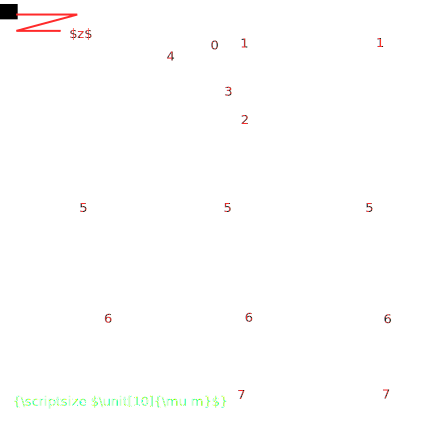
\includegraphics[width=8cm]{m_wf}
    \svginput{.6}{m_wf}
    \svginput{.6}{m_sec}
    \caption{{\bf left:} Wide field focus series of a
      three-dimensional distribution of yellow-green beads in agarose
      gel. Sampling in $z$ is $\unit[1]{\mu m}$. {\bf left:}
      Computationally sectioned images of the same sample. The
      corresponding raw images are shown in \figref{fig:m_phase} on
      page \pageref{fig:m_phase}.}
  \label{fig:m_wf}
\end{figure}

In those cases \cma{optical sectioning} it is useful to utilize
structured illumination to separate out-of-focus and in-focus
fluorescence. The mosaic on the right of \figref{fig:m_wf} shows the
computed optical sections from four raw images per slice, which are
displayed in \figref{fig:m_phase} in the appendix on page
\pageref{fig:m_phase}.  The sections contain relatively distinctive
vertical reconstruction artifacts. These can be avoided using the HiLo
reconstruction method which has the additional advantage of only
needing two raw images per slice.

However, \cma{bead localization} the HiLo method needs considerably
more code and I have not implemented it in my real-time imaging
software. Also, the artifacts have no effect on the localization
precision of the algorithm that I describe next: I determine the
center of each bead by finding local maxima after applying a
three-dimensional difference of Gaussian filter (matched to the bead
diameter). The result is depicted in the inlay in \figref{fig:m_ang}.

% \begin{figure}[hbtp]
%   \centering
%   \svginput{.7}{m_sec}
%   \caption{}
%   \label{fig:m_sec}
% \end{figure}
Im naechsten Schritt werden die einzelnen Beads individuell
beleuchtet, indem eine helle Scheibe an der entsprechenden Stelle des
focal plane SLM angezeigt wird. Gleichzeitig wird auf dem pupil plane
SLM jeweils eine Maske dargestellt die die Beleuchtung der
out-of-focus beads verhindert. Die Maske wird automatisch mit einem
Raytracer aus dem dreidimensionalen Modell der Beadverteilung
berechnet. 


\begin{figure}[hbtp]
  \centering
  \svginput{1}{angular-beads}
  \caption{Spatio-angular controlled illumination of the beads from
    \figref{fig:m_sec}. The top left image shows bead number zero and
    so forth, the second image in the top shows bead number one and so
    on. The LCoS selectively illuminates the target bead and the MMA
    displays the pattern shown in \figref{fig:m_bfp_co}.}
  \label{fig:m_ang}
\end{figure}

Die acht Kamerabilder mit den einzelnen Beads sind in den oberen zwei
Zeilen von \figref{fig:m_ang} dargestellt. Im Gegensatz zu
\figref{fig:m_wf} ist hier keine Fokusserie gezeigt, sondern auf jeden
Bead wurde einzeln fokussiert. Die entsprechenden pupil plane SLM
Masken sind darunter dargestellt. Den \cma{description of pupil plane
  masks} Aufbau der Maske moechte ich kurz and der Aufnahme von Bead 4
erlaeutern. An der 3D Darstellung im Inlay in \figref{fig:m_ang} sieht
man, dass bead 4 sich am Rand der Verteilung befindet und alle anderen
beads auf nur auf einer Seite von ihm. Der Winkel zwischen der
Verbindungsgerade von bead 4 und bead 6 bezueglich der optischen achse
ist der kleinste. Daher entspricht der in der Maske mit einem Pfeil
markierte einzelne ``Schatten'' bead 6. Alle anderen beads wuerden nur
beleuchtet werden wenn bead 4 unter extrem hohem Winkel angeleuchtet
wird. Sie fallen in den zweiten Schatten am Rand der Pupille.

Wenn \cma{stability} man sich die Bilder in
\figref{fig:m_ang} genauer betrachtet, dann faellt zunaechst auf, dass
die Bilder fuer bead 2 und 7 komplett dunkel sind. Das liegt daran,
dass das sich mapping zwischen Kamera und focal plane SLM zwischen
Kalibration mit einem fluorescent plane sample und der Messung mit den
beads um wenige microns verschoben hat. Bead 6 wird exakt
angeleuchtet, aber bei Bead 5 und 3 weicht die Beleuchtung zunehmend
ab. Nach der Messung wurden die Gummifuesse vom Mikroskop entfernt und
der Mikroskopkoerper auf dem Metalltisch verschraubt und derartige
Probleme traten nicht mehr auf.

Ein \cma{artifacts} interessanteres Problem sieht man, wenn man sich
das Bild von Bead 5 genau anschaut. Dort sieht man das nur die untere
Haelfte des Beads beleuchtet ist. Durch die Hintergrundfluoreszenz des
Agarose Gels sieht man aber auch den runden Bereich, der durch den
focal plane SLM angeleuchtet wird. Fuer manche Sample wird es dadurch
vermutlich schwierig mehrere focal plane Belichtungen seamless
ineinanderuebergehen zu lassen und Bilder wie in einem konfokalem
Mikroskop zu erzeugen.

Ich \cma{comparison spatial control and only angular control} habe die
Bilder in \figref{fig:m_ang} sowohl mit vollen Beleuchtungswinkeln
aber auch mit der Winkelkontrolle.  Bei der selektiven Beleuchtung
einzelner Beads hat sich die Hintergrundfluoreszenz in den Bildern
erheblich verringert. Leider kann man keine Verbesserung feststellen,
wenn man dann auch noch die Winkelkontrolle zuschaltet. Ich denke dies
kann man durch die hohe Hintergrundfluoreszens des Agarose Gels und
die geringe Dichte an Beads erklaeren. Nur dass man die Fluoreszens
von Out-of-focus beads nicht mehr im Rauschen nachweisen kann,
bedeutet jedoch nicht, dass die Winkelkontrolle nicht doch einen
positiven Effekt hat. Schliesslich wird vermieden, dass die Beads
nutzlos angeregt werden. Man kann es eben nur schwer nachweisen.

\section{Winkelbeleuchtung in hoeherer Konzentration an Beads}

Um den Einfluss der Winkelkontrolle der Beleuchtung direkt zu messen
habe ich ein weiteres Sample mit einer hoeheren Konzentration an Beads
in anderem Agarose Gel mit deutlich geringerer Eigenfluoreszens
angefertigt.

\begin{figure}[!hbt]
  \centering
  \svginput{1}{montage-ang}
  \caption{}
  \label{fig:montage-ang}
\end{figure}


In \figref{fig:montage-ang} sind die entsprechenden Aufnahmen
dargestellt. Im wide field Bild ist mit einem weissen Kreis mit
gestrichelter Linie der Bead dargestellt, der dann durch den focal
plane SLM selektiv angeleuchtet wird. 

Der Einfachheit halber habe ich hier auf die Beleuchtungsoptimierung
mittels Raytracer verzichtet und variiere mit der Geometrie wie in
\figref{fig:overview-bleach}~e) ein rundes Fenster ($\rho=0.7, r=0.3$)
auf dem pupil plane SLM.

Die Bilder im Mosaik auf der rechten Seite von \label{fig:montage-ang}
zeigen die 100fach verstaerkte Intensitaet des linken unteren Bildes
und der mit der Fensterposition variierende Beleuchtungskegel macht
sich als Aenderung der relativen intensitaet der out-of-focus beads
bemerkbar. Ein deutlicher Unterschied ist beispielsweise zwischen dem
Bild fuer $\theta=30^\circ$ und $\theta=330^\circ$ an der mit einem
Pfeil markierten Stelle zu erkennen.

\section{Conclusion}
Die beschriebenen Experimente zeigen, dass die Hardware des Mikroskops
prinzipiell funktioniert.  Insbesondere fuer den in section
\ref{sec:beads_under} beschriebenen Versuch musste eine grosse Menge
an Software kombiniert werden, um Kamera und focal plane SLM zu
kalibrieren, die beads zu lokalisieren, optimale Beleuchtungspattern
zu erzeugen und dies alles mit der Hardwaresteuerung zusammen laufen
zu lassen, so dass das gesamte Experiment moeglichst automatisch und
in ueberschaubarer Zeit ablaeuft.

Das Hauptproblem und der groesste Zeitaufwand lag hier vor allem an
nicht ausreichenden Informationen ueber einige der nicht ersetzbaren,
alternativlosen Hardwarekomponenten.

%%% Local Variables: 
%%% mode: latex
%%% TeX-master: "kielhorn_memi"
%%% End: 

\chapter{Discussion}
\label{sec:discussion}
The aim of this thesis has been the development of a wide-field
fluorescence microscope system that can control the irradiance in the
specimen as well as the illumination angles with the aim of decreasing
phototoxicity.

The original \cma{origin of the idea} idea was to combine a
programmable array microscope with control of the illumination
directions. Initially this seemed to be an elegant approach: The
programmable array microscope produces two images on a camera, one of
which contains only out-of-focus light. By variation of the
illumination angle of the excitation light, it should be possible to
find the direction with minimal out-of-focus contributions.
 
Fairly quickly it became clear that this approach, if at all, would
work only inefficiently. After all, for the programmable array
microscope to work, fine structures must be imaged into the
specimen. This, however, has the consequence that several diffraction
orders instead of just one bundle of rays must traverse the
sample. For most specimens this will bring no advantage compared to a
wide-field microscope.

We opted instead for a modification of the excitation path in a
wide-field microscope. My assumption was that given an estimate of the
three-dimensional fluorophore distribution, and perhaps additional
information about the expected movement of cells, pathogens or organs;
a sufficiently accurate prediction of the expected out-of-focus light
can be made.

Using \cma{description of the hardware} two spatial light modulators
(SLM), we can project appropriate distributions of excitation light
into the sample. One SLM controls the angle and the other the in-focus
pattern of light. Our goal for was to acquire one stack, consisting of
twenty slices, per minute. For this, partial recordings of slices
should be acquired in sequence and later composed into one image (see
chapter \ref{sec:concept}, in particular section
\ref{sec:illum-opt}). Therefore we selected the SLM devices with an
emphasis on high speed.

The fastest commercially available SLMs are ferroelectric liquid
crystal on silicon devices (fLCoS) and digital micromirror devices
(DMD), both of which can only do binary modulation. However, in our
case binary intensity modulation is disadvantageous. Sharp edges lead
to high diffraction losses and strong oscillations of the field in the
Fraunhofer diffraction pattern.

\nomenclature{fLCoS}{Ferroelectric liquid crystal on silicon device, a
  reflective spatial light modulater based on switching liquid
  crystals between two bistable states. It is a particularly fast
  technology.}

The pupil \cma{Why Fraunhofer micromirror array?} plane SLM, that
controls the illumination angles should ideally not be a binary
device, otherwise oscillations of excitation intensity would occur in
the specimen and appear on the camera image. For this reason, we use a
specifically developed SLM, which resembles a DMD in terms of mode of
operation and speed but can display gray scale values.  A $256\times
256$ mirror array suffices for angular control. This facilitated the
development of the mirror and fast control electronics at Fraunhofer
IPMS.

The focal plane SLM, on the other hand, should have a high resolution
\cma{choice for focal plane SLM} and it should be possible to update
its patterns very fast, so that the illumination can be adapted to the
specimen during acquisition with low latency. Initially I opted for a
SLM that is connected to the graphics card of a computer. We chose a
fLCoS SLM because its pixel borders are less sharp than those of the
DMD and we expected a better efficiency for our
application. Unfortunately, there were difficulties with the
synchronization between the graphics card and the other
devices. Therefore, relatively late into the project {\color{red}
  FIXME is that an okay expression?}, I had to replace the SLM
controller with another one that contains internal memory and is
linked to a computer via USB.  \nomenclature{USB}{Universal Serial
  Bus.}  Unfortunately, the USB connection is very slow and fast
update of image patterns is no longer possible. In retrospect, it
would have been easier to use two of the custom-made grey value SLMs
from Fraunhofer. Note that Institut Pasteur and Fraunhofer IPMS
continue this work and do just that under the Joint-Programme Inter
Carnot Fraunhofer PICF 2011, ``Micromirror Enhanced Microscopic
Imaging for high-speed angular and spatial light control in spectral
Optogenetics and Photomanipulation applications in biological
applications'' (MEMI-OP).

A \cma{remedy against low acceptance angle} serious disadvantage of
the Fraunhofer SLM in combination with the Fourier optical filter
approach employed in our prototype is the small acceptance angle. This
limits the exposed field to $\unit[80]{\mu m}$ diameter for a
wavelength of \unit[473]{nm} using a $63\times$ objective with a
numerical aperture of $1.4$, while the objective does support
$\unit[400]{\mu m}$ field diameter. One solution could be contrast
generation in a common path interferometer as described in the patent
application \citep{Heintzmann2010a}. The approach is derived from
reflective Nomarski differential interference contrast microscopy. A
birefringent prism separates the illumination bundle into bundles that
have a small offset (shear).  If the shear distance corresponds to the
pixel pitch $\Lambda=\unit[16]{\mu m}$ of the micromirrors then this
device converts height differences between adjacent mirrors into
intensity contrast. My experiments with a set of Nomarski prisms that
were available in our lab showed that this method can work. However,
the prisms had too small a shear angle and returning diffraction
orders were cut off. Meanwhile planning for the original, and with
respect to acceptance slightly flawed, prototype had advanced so far
that the change of the contrast method no longer seemed possible and
the project consortium decided to abandon the development of this
alternative contrast method. However, the common path interferometer
is still a very promising method and has the potential for good
contrast at large acceptance angles when prisms with larger shear
angles are used. Additionally, it should be noted that this
interferometric method will work better when using piston-type
micromirrors as compared to torsion micromirrors.

Given \cma{priority of the control algorithm} the \emph{low
  transmission} of our prototype, which could be just barely enough to
investigate the biological test system of \celegans\ embryos, the
disproportionally high effort that went into synchronizing the two
fast SLMs which can only run at a \emph{reduced duty cycle}, and the
\emph{limited etendue} which excludes some interesting experiments, it
would have been better in hindsight, to build a demonstrator with two
slow, conventional, grey-value SLMs and to spend more effort on the
development of the illumination control algorithm and biological
experiments.

In \cma{holographic system} this context, with the aim of simplifying
the hardware, I built a holographic illumination system consisting of
a single phase-only SLM in the intermediate image plane. This enables
the simultaneous control of both the in-focus light distribution as
well as the illumination angles in the specimen. The SLM displays
diffraction gratings and its arrangement is such, that the first
diffraction order illuminates the pupil. The illumination angle in the
specimen can be adjusted by the grating period and direction while the
local irradiance is controlled with the grating contrast.


  % - holographie loest jedoch nicht das problem geringer ettendue (die moegliche
  %   ettendue muss ich mir genauer ueberlegen, sie haengt mit der
  %   anzahl der pixel des displays und den grating konstanten zusammen,
  %   die dargestellt werden koennen, da das system off-axis betrieben
  %   werden muss, wird die ettendue geviertelt)

Unfortunately the phase-only SLM that I used for the experiments
suffers from cross-talk between pixels, a non-linear transfer function
and temporal fluctuations of the displayed phase pattern. It was
uncertain whether these problems could be circumvented. Especially
higher orders which are generated by the device's non-linearity are a
problem when they reach the sample. Furthremore, it seems particularly
difficult to project a grating with small period into the sample
because this requires the superposition of two phase gratings on the
SLM --- a formidable task in the light of its  FIXME probleme.

Projecting grating patterns is necessary, because for my illumination
algorithm I need a reasonably good measurement of the
three-dimensional fluorophore distribution. For many specimen
structured illumination is necessary to remove out-of-focus light from
the raw images and obtain optical sections. Other phase SLMs which
became available more recently have a much better performance and
could presumably be used to construct a holographic spatio-angular
illumination device.

The \cma{sectioning by structured illumination} main prototype of our
project with two SLM, as described in chapter \ref{sec:dev1}, is more
suitable for structured illumination. The period on the focal plane
SLM and the illumination aperture defined by the pupil plane SLM can
be selected for best possible contrast of the in-focus light
pattern. Optically sectioned images can then be calculated with
various methods. The HiLo method proposed by Jerome Mertz and best
documented in \cite{Mertz2010} is preferable to others as only two
exposures per slice are necessary. Since images in our system are
taken in rapid succession and movement artifacts are unlikely, we
developed a variant of the HiLo method. In contrast to the original,
which uses one uniformly illuminated image and one with structured
illumination, we use two structured illumination images leading to an
improved signal-to-noise ratio.

During my work on the project \cma{sCMOS --- new camera technology} a
much improved camera technology (sCMOS) came to market. No such camera
was used for measurements in this work. It could, however, be added to
our system without substantial changes.

I use \cma{Arduino for control electronics} an Arduino microcontroller
for electronic synchronization. This cheap and easy to use electronics
platform has been used for several years in our lab and is
particularly useful for synchronization of multiple devices. The
source code for the Arduino microcontroller is often short and
relatively easy to read. This controller is thus well suited to
document the logic in our synchronization circuits and can be easily
understood and extended by new members of our group.

During this work, I used many different electronic devices (SLM:
Hamamatsu, Holoeye, ForthDD, Texas Instruments, Fraunhofer, cameras:
Andor (Clara, IXon2, IXon3, IXon Ultra, Neo sCMOS), Photometrics
Cascade II, Hamamatsu (Orca Flash 2.8 and 4.0), Logitech Pro 9000, and
more). I noticed that construction and debugging effort depend very
much on the quality of the documentation. If documentation is
insufficient, which unfortunately is often the case, then it helps if
communication is done with open standards (USB video device class,
Ethernet).

Particularly positively I was surprised by the Texas Instruments
DMD. The SLM development kit (DLP LightCrafter, YoungOptics) is very
mature \citep{Guide2012}, contains open source software and high
quality documentation explaining even the control registers of
individual chips.

Unlike the Fraunhofe micromirror array (as described in section
\ref{sec:mma}), the Texas Instruments digital micromirrors tilt around
their diagonals. For the 0.3~WVGA DMD, that is used in my development
kit, the pixels are addressed in a diagonal pattern but can be
illuminated parallel to one of the edges of the device. This
simplifies building the setup at the expense of a slightly more
complicated software control. The larger DMD devices can be addressed
more easily but must be illuminated in an angle of $45\degree$
relative to the device.

While working with the kit I was able to implement
features within three days, for which I spent several months of
reverse engineering and trial and error on devices of other
manufacturers --- most notably, controlling individual frames at the
fastest possible update rate (1440 frames per second) via HDMI. If I
had known this before, I would have designed the prototype differently
and I would have accepted some drawback regarding optical performance.


I \cma{Open hardware is a good thing} am not content with the current
state of scientific cameras because all of them gave me problems with
incompatible or unstable drivers. Therefore, I hope that there will be
more projects that open their resources to the public, such as Marc
Levoy's Franken Camera \citep{Adams2010}; or that the manufacturers of
the ever-improving consumer cameras document and disclose the
protocols for disabling automatic image processing and accessing raw
sensor data for their devices (as with the Logitech Pro 9000).


%Fu2011

Both our \cma{results of existing control software} prototype and the
software for illumination optimization have been designed for the
observation of cells in a developing \celegans\ embryo. So far, I was
able to demonstrate spatio-angular illumination on static, non-living
samples but I have not yet applied the method on living
organisms. Here, the main problem is that the image upload, especially
to the focal plane SLM, takes disproportionally long.

\section{Outlook}

If \cma{proposition for an optogenetics experiment} the sample does
not change very fast, and plenty of time is available to upload images
into the SLM controllers, then the current prototype allows
experiments with rapidly changing illumination patterns (about 1000
fps is attainable). One interesting biological experiment would be
similar to \cite{Branco2010}. There, synapses were excited by moving a
focal spot along one linear dendrite and its response was recorded as
a function of the speed of the focal spot. With our system, two
branches of a dendrite could be stimulated simultaneously. Thereby,
the response of the junction could be investigated.

The \cma{next steps for control software} algorithm for the
optimization of the illumination patterns can still be improved. So
far, I assume that the sample can be represented well by spheres. The
nuclei in each slice are illuminated individually and the algorithm
finds illumination angles so that exposure of out-of-focus nuclei is
avoided. An obvious improvement would be to find nuclei that can be
illuminated with similar angles and group them for simultaneous
exposure. Even better would be an algorithm in which the specimen is
not represented as solid bodies but works directly on stacks of
optical sections. In a first simple experiment, using the
computational power of graphics processing units, I could show that
the extensive calculations can be carried out in reasonable time
frames. (FIXME maybe mention this in in main text and add appendix)

\cma{maximum likelihood deconvolution} 

Weitere Untersuchungen zur Datenauswertung waeren sehr nuetzlich. Wie
bereits in \ref{sec:pam} angedeutet, koennte man unter Kenntnis des
Mappings zwischen focal plane SLM und Kamera ein und der SLM pattern
ein komputerisiertes Descanning umsetzen, also eine Klassifizierung
der Rohbilddaten in in-focus und out-of-focus photonen. Dafuer waere
jedoch vermutlich ein genaueres Verstaendnis der Lichtverteilung im
Sample notwendig.
 In diesem zuammenhang waere es hilfreich zu simulieren.

 \cma{partial coherent simulation}  It would be interesting to simulate the
wave-optical image formation of the prototype with partial
coherence. This would answer the question how important the grey
levels of the micromirror array in the pupil-plane really are, and
whether or not we can replace it with a binary DMD.

A similar simulation should be used to investigate the influence of
field mask B0 and Fourier stop B1 on the contrast and the transfer
function of the schlierenoptics system.




% - eine genaue analyse einiger probleme mit wellenoptischer partiell
%   kohaerenter theorie steht noch aus und waere interessant (nach
%   wichtigkeit)

%   - partiell kohaerente simulation des mma im schlierenoptischen system

%     - sind graulevel vorteilhaft?

%     - wuerde ein mma, bei dem alle spiegel in dieselbe richtung kippen
%       die ettendue verdoppeln?

%   - partiell kohaerente simulation des mma im shearing
%     interferometrischen system

%     - was ist die maximale ettendue eines wollaston prismas?

%   - holographie methode mit extended source

  % - Denkbar waere auch ein scannendes konfokales Mikroskop, dass an
  %   die Beleuchtungswinkel an jedem Punkt kontrolliert (siehe
  %   fig:hourglass-all-b).  Bisher wurden in der Literatur nur Systeme
  %   beschrieben, die die Phase des Beleuchtungslicht in der Pupille
  %   aendern (FIXME ref). Eine Adaption dieser Systeme zu einem
  %   spatio-angularen ist naheliegend und ich schlage vor, derartige
  %   Systeme auch untersucht werden sollten. Die Kombination von CLEM,
  %   einem Ringdetektor (vielleicht mit UZI) koennte die Bildgebung im
  %   Inneren lebender Organe (z.B. Gehirn) verbessern.

\appendix
\chapter{EM-CCD camera calibration}
\section{Andor Basic code listing for automatic image acquisition}
\label{sec:basic-acquisition}
\definecolor{light-gray}{gray}{0.95}

\lstdefinestyle{myframe}{
  basicstyle=\LSTfont,
  % basicstyle=\footnotesize\ttfamily,
  rulesepcolor=\color{gray} ,
  rulecolor = \color{black},
  frame = single,
  % framerule = 0pt,
  backgroundcolor =\color{light-gray}, 
  fontadjust=true,
  breaklines = true,
  showstringspaces=false,
  commentstyle=\itshape,
}
\lstdefinestyle{mymaxima}{
  language=C,
  style=myframe
}
\lstdefinestyle{myclang}{
  language=C,
  style=myframe
}
\lstdefinestyle{myfortran}{
  language=Fortran,
  style=myframe
}
\lstdefinestyle{mymatlab}{
  language=Matlab,
  style=myframe
}
\lstdefinestyle{mylisp}{
  language=Lisp,
  style=myframe
}
\lstdefinestyle{mybasic}{
  language=[Visual]Basic,
  style=myframe
}
\lstdefinestyle{mypython}{
  language=Python,
  showstringspaces=false,
  tabsize=4,
  basicstyle=\ttfamily,
  morekeywords={models, lambda, forms},
  frame = single,
  breaklines = true,
  style=myframe
}


\begin{lstlisting}[style=mybasic]
' This is code for the Basic interpreter in Andor Solis
function ~GetSaturatingExposure()
        SetKineticNumber(1)
        exp=.01
        SetExposureTime(exp)
        run()
        m=maximum(#0,1,512)
        GetSaturatingExposure=exp*10000/(m-100)
        CloseWindow(#0)
return
name$ = "C:\Users\work\Desktop\martin\20111111\scan-em3\ixon_"
print("start")

SetOutputAmp(1)
print("conv_start")
exp= ~GetSaturatingExposure()
print(exp)
SetExposureTime(exp)
SetKineticNumber(20)
SetShutter(0,1)
run()
save(#0,name$ + "conv1_dark.sif")
ExportTiff(#0, name$ + "conv1_dark.tif", 1, 1, 0, 0)
CloseWindow(#0)
CloseWindow(#1)
        
SetShutter(1,1)
run()
save(#0,name$ + "conv1_bright.sif")
ExportTiff(#0, name$ + "conv1 _bright.tif", 1, 1, 0, 0)
CloseWindow(#0)
CloseWindow(#1)

SetOutputAmp(0)
SetShutter(1,1)
for i = 40 to 300 step 10
        SetGain(i)
        exp=~GetSaturatingExposure()
        print(exp)
        SetExposureTime(exp)
        SetKineticNumber(20)
        SetShutter(0,1)
        run()
        save(#0,name$ + str$(i) + "_dark.sif")
        ExportTiff(#0, name$ + str$(i) + "_dark.tif", 1, 1, 0, 0)
        CloseWindow(#0)
        CloseWindow(#1)
        SetShutter(1,1)
        run()
        save(#0,name$ + str$(i) + "_bright.sif")
        ExportTiff(#0, name$ + str$(i) + "_bright.tif", 1, 1, 0, 0)
        CloseWindow(#0)
        CloseWindow(#1)
next

SetOutputAmp(1)
print("conv_end")
exp= ~GetSaturatingExposure()
print(exp)
SetExposureTime(exp)
SetKineticNumber(20)
SetShutter(0,1)
run()
save(#0,name$ + "conv2_dark.sif")
ExportTiff(#0, name$ + "conv2_dark.tif", 1, 1, 0, 0)
CloseWindow(#0)
CloseWindow(#1)
        
SetShutter(1,1)
run()
save(#0,name$ + "conv2_bright.sif")
ExportTiff(#0, name$ + "conv2 _bright.tif", 1, 1, 0, 0)
CloseWindow(#0)
CloseWindow(#1)
\end{lstlisting}

\begin{table}[!htbp]
  \centering
%  \begin{tabular}{|l|l|l|l|l|l|l|l|}
  \begin{tabular}{r l l r  l r l}
\hline
$\textsf{gain}_\textrm{software}$ & $1/(M\cdot M_\textrm{pre})$ & $N_r$ & $N_{(M)}/(W\times H)$ &  \textsf{exposure} & $N_{(M)}'/(W\times H)$ & $1/F_n$ \\
 & [e/ADU] & [e/px] & [e/px] & [ADU] & [s] & [e/(px s)]  \\
\hline
conv1 & 1.3165 & 7.189 & 3008.66      & 0.2016 & 14923 & 0.981 \\
50 & 0.1160 & 0.486 & 260.05 & 0.0289 & 8995 & 0.591 \\
60 & 0.0984 & 0.406 & 225.46 & 0.0249 & 9054 & 0.595 \\
70 & 0.0841 & 0.349 & 190.52 & 0.0212 & 8983 & 0.591 \\
80 & 0.0729 & 0.305 & 165.24 & 0.0186 & 8907 & 0.586 \\
90 & 0.0680 & 0.288 & 150.54 & 0.0161 & 9368 & 0.616 \\
100 & 0.0611 & 0.262 & 128.47 & 0.0136 & 9427 & 0.620 \\
110 & 0.0550 & 0.241 & 121.11 & 0.0129 & 9409 & 0.619 \\
120 & 0.0510 & 0.228 & 113.71 & 0.0120 & 9498 & 0.624 \\
130 & 0.0465 & 0.211 & 106.66 & 0.0112 & 9541 & 0.627 \\
140 & 0.0433 & 0.201 & 96.95 & 0.0101 & 9564 & 0.629 \\
150 & 0.0405 & 0.192 & 89.68 & 0.0093 & 9671 & 0.636 \\
160 & 0.0380 & 0.183 & 87.24 & 0.0090 & 9656 & 0.635 \\
170 & 0.0359 & 0.175 & 81.56 & 0.0084 & 9739 & 0.640 \\
180 & 0.0339 & 0.169 & 79.80 & 0.0081 & 9863 & 0.648 \\
190 & 0.0321 & 0.163 & 74.00 & 0.0075 & 9806 & 0.645 \\
200 & 0.0305 & 0.158 & 72.57 & 0.0073 & 9878 & 0.649 \\
210 & 0.0292 & 0.155 & 69.44 & 0.0070 & 9944 & 0.654 \\
220 & 0.0280 & 0.150 & 67.69 & 0.0068 & 9971 & 0.656 \\
230 & 0.0268 & 0.147 & 65.63 & 0.0065 & 10057 & 0.661 \\
240 & 0.0257 & 0.188 & 63.90 & 0.0063 & 10131 & 0.666 \\
250 & 0.0244 & 0.140 & 62.52 & 0.0062 & 10026 & 0.659 \\
260 & 0.0237 & 0.137 & 62.86 & 0.0062 & 10078 & 0.663 \\
270 & 0.0229 & 0.135 & 63.17 & 0.0062 & 10130 & 0.666 \\
280 & 0.0221 & 0.133 & 63.64 & 0.0062 & 10204 & 0.671 \\
290 & 0.0214 & 0.130 & 63.38 & 0.0062 & 10162 & 0.668 \\
300 & 0.0205 & 0.128 & 63.20 & 0.0062 & 10133 & 0.666 \\
conv2 & 1.5953 & 8.768 & 8198.86 & 0.5291 & 15496 & 1.019 \\
\hline
\end{tabular}
%  \includegraphics[width=12cm]{../app_cam/ixon3}
\caption{Comparison of read noise for different EM-gain settings
  (first column) of the Andor IXon3. $W$ and $H$ are the size of the sensor (in pixels). The value $N_{(M)}'$
  estimates the number of photoelectrons the detector would have
  seen with \unit[1]{s} integration time and is used to calculate
  the excess noise factor in the last column. In EM-mode the fastest
  readout speed was used \unit[10]{MHz} with vertical shift speed of
  \unit[1.7]{$\mu$s}.}
  \label{tab:ixon-table}
\end{table}

\newpage

\section{Python code listing for the read noise evaluation}
\label{sec:python-readnoise-eval}

\begin{figure}
  \centering
  \pdfinput{17cm}{ixon_conv1}
  \pdfinput{17cm}{ixon_300}
  \caption{Readnoise evaluation using the Python code in section
    \ref{sec:python-readnoise-eval}{\bf top:} Conventional readout of
    an Andor IXon3 camera. {\bf bottom:} readout with an EM-gain
    setting of 300 on the same camera with identical sample. {\bf
      left:} 2D histogram of per pixel variances against binned
    intensities. {\bf middle:} variance of 20 dark images. {\bf
      right:} mean of 20 dark images.}
  \label{fig:ixon}
\end{figure}
  


\begin{lstlisting}[style=mypython]
#!/usr/bin/env python
# ./ti.py /media/backup/andor-ultra-ixon/martin/20111111/scan-em3/ ultra 2700
import sys
import os

import matplotlib
matplotlib.use('Agg')

from pylab import *
from libtiff import TIFFfile, TIFFimage
from scipy import stats

seterr(divide='ignore')

folder = sys.argv[1]
cam = sys.argv[2]
gain = sys.argv[3]

def readpics(gain,cam='ixon_',isdark=False):
    print 'loading ', os.path.join(folder,cam) + '_' + gain + '_bright.tif'
    fg=TIFFfile(os.path.join(folder,cam) + '_' + gain + '_bright.tif')
    bright,bright_names=fg.get_samples()
    bg=TIFFfile(os.path.join(folder,cam) + '_' + gain + '_dark.tif')    
    dark,dark_names=bg.get_samples()
    return (bright[0],dark[0])

(f,b) = readpics(gain=gain,cam=cam)

bg=mean(b,axis=0)
v=var(f,axis=0)
i=mean(f,axis=0)

ny,nx=64,128
H,y,x=histogram2d(v.flatten(),i.flatten(),bins=[ny,nx],
                  range=[[0,v.max()],[0,i.max()]])
extent = [x[0], x[-1], y[0], y[-1]] 
acc=zeros(x.shape,dtype=float64)
accn=zeros(x.shape,dtype=int64)
s=nx/i.max()
for ii,vv in nditer([i,v]):
    p=round(ii*s)
    acc[p]+=vv
    accn[p]+=1   

fig=figure(figsize=(24, 8),dpi=300)
hold(False)
title('bal')
subplot(1,3,1)
imshow(log(H), extent=extent,
           aspect='auto', interpolation='none',origin='lower')
hold(True)
ax=x[nonzero(accn)]
ay=acc/accn
ay=ay[nonzero(accn)]
l=round(.6*len(ax))
bx=ax[0:l]
by=ay[0:l]
plot(ax,ay,'r+')
slope,intercept,rval,pval,stderr=stats.linregress(bx,by)
plot(ax,polyval([slope,intercept],ax))
xlabel('intensity/ADU')
ylabel(r'variance/ADU$^2$')
real_gain=1/slope # unit electrons/ADU
read_noise=sqrt(var(b))*real_gain # electrons RMS per pixel
mean_elecs=(mean(f)-mean(b))*real_gain # photoelectrons electrons per pixel
print gain,cam,real_gain,read_noise,mean_elecs,mean(b),rval,pval,stderr
tit='EM-gain: %s, cam: %s, real gain: %.2f e/ADU\n
read noise: %.2f e RMS/pixel, mean: %.2f e/pixel, offset: %.2f'
% (gain,cam,real_gain,read_noise,mean_elecs,mean(b))
title(tit)
subplot(1,3,2)
imshow(var(b,axis=0))
title('variance of darkimages')
colorbar()
subplot(1,3,3)
imshow(mean(b,axis=0))
title('mean of darkimages')
colorbar()
show()
fig.savefig(cam+'_'+gain+'.png')
\end{lstlisting}


\chapter{Optical sectioning by structured illumination}
\comment{
\jpginput{}{m_phase}{}
}


\begin{figure}[H]
  \centering
  
\includegraphics[height=.6\textheight]{m_phase}
  \caption{Structured illumination images of the same of the beads
    from \figref{fig:m_wf}. Of each $z-$slice (rows) four exposures
    with different grating phase (columns) were captured.}
  \label{fig:m_phase}
\end{figure}


\chapter{Mapping between focal plane SLM and camera}
\label{sec:app_map}
\section{Rigid coordinate transformation}
Each term of the sum in equation
\ref{eqn:rigid-sum} on page \pageref{eq:rigid-sum} can be expressed as
two scalar terms:
\begin{align}
  \mathcal{Q}=\sum_i^n&
  \abs{s(\cos\phi r^c_{ix}+q\sin\phi r^c_{iy})+t_x-r^d_{ix}}^2
  +
  \abs{s(-\sin\phi r^c_{ix}+q\cos\phi r^c_{iy})+t_y-r^d_{iy}}^2
\end{align}

The following Maxima code will find the solution to the least squares
problem:
\begin{lstlisting}[style=mymaxima]
load(minpack)$
q:-1;
g(s,p,tx,ty):=[s*( cos(p)*<cx>+q*sin(p)*<cy>)+tx-<dx>,
               s*(-sin(p)*<cx>+q*cos(p)*<cy>)+ty-<dy>, ... ]$
minpack_lsquares(g(s,p,tx,ty), [s,p,tx,ty], [0.88,-3.1,1200,-20]);
\end{lstlisting}
I define the function \verb!g! to contain all the terms of the sum.
This can easily written by a program that constructs the lines
according to the given pattern, replacing \verb!<cx>!, \verb!<cy>!
with camera coordinates and \verb!<dx>!, \verb!<dy>! with display
coordinates.
\comment{$}
The function \verb!minpack_lsquares! calls the subroutine \verb!lmder!
which was originally developed for the Fortran\footnote{Rather than
  calling a Fortran library Maxima calls a version of this function
  that was automatically translated into Common Lisp via {\sf f2cl}.}
package \verb!minpack!.

\begin{lstlisting}[style=myfortran]
c     subroutine lmder (http://www.netlib.org/minpack/lmder.f)
c     the purpose of lmder is to minimize the sum of the squares of
c     m nonlinear functions in n variables by a modification of
c     the levenberg-marquardt algorithm. the user must provide a
c     subroutine which calculates the functions and the jacobian.
c     the subroutine statement is
c       subroutine lmder(fcn,m,n,x,fvec,fjac,ldfjac,ftol,xtol,gtol,
c                        maxfev,diag,mode,factor,nprint,info,nfev,
c                        njev,ipvt,qtf,wa1,wa2,wa3,wa4)
\end{lstlisting}
The reason for using Maxima is, that it calculates the symbolic
Jacobian for the problem. This makes it straight forward to change the
simple rigid transform to a model with more parameters.

The following Common Lisp code shows how the result of the
optimization can be used to initialize the OpenGL modelview matrix to
transform objects in its buffer, so that they will appear at the given
positions on the camera.
 
\begin{lstlisting}[style=mylisp]
(defun load-cam-to-lcos-matrix (&optional (x 0s0) (y 0s0))
  (let* ((s 0.828333873909549) (sx  s)        (sy  (- s))
         (phi -3.102)          (sp (sin phi)) (cp (cos phi))
         (tx 608.433)          (ty 168.918)
         (a (make-array (list 4 4) :element-type 'single-float
             :initial-contents
             (list (list (* sx cp)    (* sy sp)  .0   (+ x tx))
                   (list (* -1 sx sp) (* sy cp)  .0   (+ y ty))
                   (list .0           .0        1.0   .0)
                   (list .0           .0         .0  1.0)))))
    (gl:load-transpose-matrix (sb-ext:array-storage-vector a))))    
\end{lstlisting}  
Alternatively, here is the equivalent code in C (with different
parameters):

\begin{lstlisting}[style=myclang]
float m[4*4]; // OpenGL Modelview Matrix
float s=-.8749328910202312,
      sx=s,sy=-s,phi=-.8052030670943575,
      cp=cos(phi),sp=sin(phi),
      tx=1456.71806436377,
      ty=910.4787738693659;
  m[0]=   sx*cp;   m[4]=sy*sp;   m[8] =0;    m[12]=tx; 
  m[1]=-1*sx*sp;   m[5]=sy*cp;   m[9] =0;    m[13]=ty; 
  m[2]=0;          m[6]=0.;      m[10]=1;    m[14]=0;  
  m[3]=0;          m[7]=0.;      m[11]=0;    m[15]=1;  
glMatrixMode(GL_MODELVIEW);
glLoadMatrixf(m);
\end{lstlisting}
\section{Image processing: Localizing bright spots on the camera}
The following Matlab listing shows how to open the image files:
% cd /mnt/scan 

\begin{lstlisting}[style=mymatlab]
%% load the files
% 0 .. 99 spot images
% only 10..99 usable because the first are on border and not illuminated
  a = newim(1392,1040,103); for i=0:102
  % Andor's FITS format isn't read correctly
  % correct this by adding 2^15
  a(:,:,i) = 2^15 + readim(sprintf('o%03d.fits',i));
  end
\end{lstlisting}
  Of the 103 images, that are loaded into \verb!a!, the first 100
  contain spots and the image at the zero-based index 102 is the
  uniformly illuminated image shown in \figref{fig:rigid-pics} left.
  The other two images at indices 100 and 101 are two centered disks
  with different diameters and are not used here.

  \begin{lstlisting}[style=mymatlab]
    bright = squeeze(a(:,:,102)); % histogram of uniformly illuminated
    % image has minimum at 800 ADU
    mask = gaussf(bright,8) > 800; % create mask with illuminated area
    bg = 510; % the background is be 510 ADU

    posmax = newim(100,2); for i = 10:99
    % correct for sample non-uniformity
    corr = (squeeze(a(:,:,i)) - bg) / bright * mask;
    % find coordinates of maximum
    [coords,vals]=findmaxima(gaussf(corr,32)); [valss,valsind] =
    sort(vals); % sort coordinates by intensity
    tmp = coords(valsind,:); % collect the maximum with highest
    posmax(i,:) = tmp(end,:); % intensity into result
    end
  \end{lstlisting}

  The DIPimage toolbox provides the function \verb!findmaxima!, that
  locates all local maxima in an image with subpixel accurac y. I
  sort the result by gray value and only use the biggest.  The
  measured 100 camera coordinate pairs in \verb!posmax! correspond to
  $\r^c_i$ in equation \ref{eq:rigid-sum}.
 
  From Matlab I create the file \verb!fit.max! with batch commands
  for Maxima. Then I run Maxima. When it is finished after a few
  seconds, the file \verb!max.out! will contain the four fitted
  parameters.
 
\begin{lstlisting}[style=mymatlab]
    c = double(posmax)'; cmd =
    ''; % collect equations in maxima format
    for i=10:99 dx = num2str(400+50*mod(i,10)); dy =
    num2str(500+50*floor(i./10)); cx = num2str(c(i+1,1)); cy =
    num2str(c(i+1,2)); cmd=[cmd ' s*( cos(p)*' cx '+q*sin(p)*' cy
    ')+tx-' dx ', ...  s*(-sin(p)*'cx '+q*cos(p)*' cy ')+ty-' dy ','];
    end cmd(:,end) = []; % delete last comma

% load the fitting package and start defining the merit function g
    pre = 'load(minpack)$ q:-1; g(s,p,tx,ty):=[';
% now put cmd between
% call the fitting function and store the parameters into max.out
    cod = [']$
    fit:minpack_lsquares(g(s,p,x,y),[s,p,x,y],[.88,-1.3,1200,-20]);'
    ...  'write_data(fit[1],"max.out");']

    fid = fopen('fit.max','w'); % write maxima commands into file
    fwrite(fid,[pre cmd cod]); fclose(fid);
    [max_status,max_result]=system('maxima -b
    fit.max'); % execute maxima
  \end{lstlisting}
  We load the transformation parameters back into Matlab and create
  the diagram \figref{fig:rigid-compare} to visualize, how well the
  transform matches camera and display coordinates.

 \begin{lstlisting} [style=mymatlab]
% load rigid transformation parameters from the file into matlab
  params = load('max.out')'; scale = params(1); phi = params(2); tx =
  params(3); ty = params(4);

  mirr = -1; R = [cos(phi),mirr*sin(phi); -sin(phi),mirr*cos(phi)]; T
  = [tx ty]';

  %% plot the two grids on top of each other
  mapped = zeros(100,2); for
  i=11:100 % camera coordinates into display coordinates
  mapped(i,:) = (scale*R*q(i,:)'+T)'; end

  dpos = zeros(100,2); for i=0:99 % calculate display points
  dpos(i+1,1) = 400+50*mod(i,10); dpos(i+1,2) = 500+50*floor(i./10);
  end

  hold off; plot(dpos(:,1),dpos(:,2),'.'); hold on;
  plot(mapped(11:end,1),mapped(11:end,2),'r+');
  % \end{lstlisting}

% print -depsc2 /home/martin/thesis/kielhorn/rigid/rigid-compare

\bibliographystyle{abbrvnat}
\bibliography{literature}
%\bibliography{../All}
\end{document}


%%% Local Variables: 
%%% mode: latex
%%% TeX-master: t
%%% End: 
